\documentclass[12pt,a4paper]{report}
% =====================================================================
% M.Tech Dissertation - Q&A Based Interactive Storytelling Using
% Generative AI (Anjali Madan Jha, SAKEC, January 2026)
% =====================================================================
\usepackage[utf8]{inputenc}
\usepackage{acronym}
\usepackage{amssymb}
\usepackage{wrapfig}
\usepackage{amsmath}
\usepackage{graphicx}
\usepackage{epstopdf}
\usepackage{booktabs}
\usepackage{hyperref}
\hypersetup{
    colorlinks=true,
    linkcolor=blue,
    filecolor=magenta,
    citecolor=blue,
    urlcolor=blue,
}
\usepackage{float}
\usepackage{cleveref}
\usepackage[left=3.5cm,right=2.5cm,top=2.5cm,bottom=2.5cm]{geometry}
\usepackage{lineno}
\usepackage{comment}
\usepackage{natbib}
\usepackage{multicol}
\usepackage{xcolor}
\usepackage{amsfonts}
\usepackage{rotating}
\usepackage{multirow}
\usepackage{bm}
\usepackage[toc,page]{appendix}
\usepackage{ragged2e}
\usepackage{anyfontsize}
\usepackage{caption}
\usepackage{longtable}
\usepackage{tabularx}
\usepackage{array}
\usepackage{listings}

\definecolor{codebg}{HTML}{F5F5F5}
\lstset{
  backgroundcolor=\color{codebg},
  basicstyle=\ttfamily\small\color{black!90},
  breaklines=true,
  columns=fullflexible,
  frame=single,
  framerule=0pt,
  framesep=4pt,
  captionpos=b,
  aboveskip=4pt, belowskip=4pt,
}

% =====================================================================
% Custom commands and global definitions
% =====================================================================
\newcommand{\dedicationNamea}{Anjali's Mother}
\newcommand{\dedicationNameb}{Madan Jha}

\def\mytitle{Q\&A Based Interactive Storytelling Using Generative AI}
\def\myname{Anjali Madan Jha}
\def\mydegree{MASTER OF TECHNOLOGY}
\def\branch{Computer Engineering}
\def\mysupervisor{Dr. Vidyullata Devmane}
\def\myrollno{124MTCM1008}
\def\mydep{Department of Computer Engineering}
\def\mydegreedate{JANUARY 2026}

\setlength{\parskip}{0.5em}

\begin{document}

\baselineskip=18pt plus1pt
\setcounter{secnumdepth}{3}
\setcounter{tocdepth}{3}
\pagenumbering{roman}

\newlength{\savedparskip}
\setlength{\savedparskip}{\parskip}
\setlength{\parskip}{0pt}

% Front matter
\thispagestyle{empty}
\begin{center}
    { \large {\bfseries {\mytitle}} \par}
\vspace{2\baselineskip}
    {\large \textbf{A} \par}
\vspace{0.5\baselineskip}
    {\large \textbf{DISSERTATION/REPORT} \par} % Select 
\vspace{0.5\baselineskip}
    {\textit{Submitted for Partial fulfillment of the Requirement}\\
    \textit{For the award of the degree of}}\par
\vspace{\baselineskip}
    {\large \bf \mydegree \par} 
\vspace{0.5\baselineskip}
{\large \textbf{In} \par}
\vspace{0.5\baselineskip}
    {\large \bf \branch \par} 
\vspace{0.5\baselineskip}
    {\textit{Submitted by} \par}
\vspace{\baselineskip}
    {{\large {\bf \myname}} \par}
\vspace{0.2\baselineskip}
    {\large \textbf{(Roll No. \myrollno}) \par}
\vspace{\baselineskip}
    {Under the guidance of \par}
\vspace{\baselineskip}
    {{\large \bf \mysupervisor} \par}
\vspace{0.5\baselineskip}
    {Professor \par}
\vspace{\baselineskip}
    {\begin{figure}[!h] 
	\centering
	
\includegraphics[width=35mm]{images/SAKEC_logo.png} 
     \end{figure}
    }
%{\large \vspace*{1ex}
\vspace{\baselineskip}
    {\bf \MakeUppercase{\mydep} \par}
\vspace*{1ex}
   { \bf \uppercase{SHAH \& ANCHOR KUTCHHI ENGINEERING COLLEGE } }\\
   \vspace{-0.2 \baselineskip}
    {(An Autonomous Institute Affilated to University of Mumbai) \par}
   
 {\bf \uppercase { MUMBAI - 400 088, MAHARASHTRA (India)  \par \mydegreedate }}
 \end{center}
\addcontentsline{toc}{section}{Certificate}
\thispagestyle{plain}

\begin{minipage}[c]{1mm}
            
\includegraphics[width=23mm]{images/SAKEC_logo.png} % Change 'logo.png' to the filename of your logo
        \end{minipage}
        \hfill
        % Place the institute name on the right
        \begin{minipage}[c]{126mm} % Adjusted width
            \centering
            { \bf \large {Shah \& Anchor Kutchhi Engineering College  } }\\
   \vspace{-0.01 \baselineskip}
    {(An Autonomous Institute Affilated to University of Mumbai) }
    { \bf \small {Mumbai-400 088, MAHARASHTRA (India)   } }\\
               
            
        \end{minipage}

\vspace{0.2\baselineskip}

\begin{center}
{\Large {\bf \uppercase{Certificate}}}
\end{center}
\vspace{\baselineskip}
\hrule
\vspace{2\baselineskip}

{It is my pleasure to certify that \textbf{{\myname}} worked under my supervision for the
M.Tech dissertation/Project report entitled \textbf{{\mytitle}}
and her work is of the level of requirement set up for the dissertation/Project Report in \textbf{{\branch}} by Shah \& Anchor Kutchhi Engineering College, Mumbai.}


\bigskip

\begin{tabular}{p{0.5\textwidth}p{0.5\textwidth}}
\textbf{Date:\ ………………} & \textbf{{\myname}} \\
& \vspace{-0.2\baselineskip}\textbf{Roll No: {\myrollno}}
\end{tabular}

\vspace{\baselineskip}
\textsc{}{This is to certify that the above statement made by the candidate is correct to the best of my knowledge.}\par
\bigskip
{\textbf{{\mysupervisor}} \par}
{Professor \par \mydep \par Shah \& Anchor Kutchhi Engineering College \par Mumbai – 400 088, India}


\vspace{1\baselineskip}

{The viva-voce/Oral and Practical examination of {\textbf{{\myname}}}, M.Tech in \branch,
has been held on \ ………………}

\vspace{5\baselineskip}

\begin{tabular}{p{0.35\textwidth}p{0.35\textwidth}p{0.35\textwidth}}
\textbf{External Reviewer} & \textbf{Internal Examiner} & \textbf{Guide Name}
\end{tabular}

\vspace{4\baselineskip}

\begin{tabular}{p{0.35\textwidth}p{0.35\textwidth}p{0.35\textwidth}}
\textbf{Head of Department} & \textbf{Principal} & College Seal
\end{tabular}


\bigskip
\addcontentsline{toc}{section}{Candidate's Declaration}
\thispagestyle{empty}

\begin{center}
{\Large {\bf \uppercase{Candidate's Declaration}}}
\end{center}

\vspace{\baselineskip}
\hrule
\vspace{2\baselineskip}

\justifying
\setlength{\parskip}{0.6em}

I hereby declare that the work presented in the dissertation/Project Report entitled {\textbf{{``\mytitle''}}} for partial fulfillment of the requirement for the degree of M.Tech in \branch{} and submitted to the \mydep{} at Shah \& Anchor Kutchhi Engineering College, Mumbai, is an authentic record of my own work carried out during the period from August 2025 to January 2026 under the supervision of {\textbf{\mysupervisor}}.\par
\vspace{2\baselineskip}
The matter presented in this dissertation/Project Report has not been submitted elsewhere in part or fully to any other University or
Institute for the award of any other degree.


\bigskip


\bigskip


\bigskip

{\textbf{Signature of the student \ \ \ \ \ \ }}

{Name: \myname} \par

{Roll No: \myrollno}
\addcontentsline{toc}{section}{Certificate of Plagiarism Check}
\thispagestyle{plain}

\begin{minipage}[c]{1mm}
            
\includegraphics[width=23mm]{images/SAKEC_logo.png} % Change 'logo.png' to the filename of your logo
        \end{minipage}
        \hfill
        % Place the institute name on the right
        \begin{minipage}[c]{126mm} % Adjusted width
            \centering
            { \bf \large {Shah \& Anchor Kutchhi Engineering College  } }\\
   \vspace{-0.01 \baselineskip}
    {(An Autonomous Institute Affilated to University of Mumbai) }
    { \bf \small {Mumbai-400 088, MAHARASHTRA (India)   } }\\
               
            
        \end{minipage}

\vspace{0.2\baselineskip}

\begin{center}
{\Large {\bf \uppercase{CERTIFICATE OF PLAGIARISM CHECK}}}
\end{center}
\vspace{\baselineskip}
\hrule
\vspace{0.1\baselineskip}

\begin{center}
\begin{longtable} { |p{6cm}|p{8cm}|  }
\hline
\multicolumn{2}{|c|}{\textbf{CERTIFICATE OF PLAGIARISM CHECK}} \\
\hline
Name of the Student& \myname \\ 
\hline
Title of the Dissertation/Report & \mytitle \\ 
\hline
Name of the Supervisor/Guide & \mysupervisor \\ 
\hline
Name of the Department & \mydep \\ 
\hline

Similar content (\%) identified &   ~~~~~~~  \% \\ 
\hline
Acceptable Maximum Limit &   10\% \\
\hline
Name of the Similarity tool used for Plagiarism Report &   Turnitin \\
\hline

Date of Verification &    \\ 
\hline

Name \& Sign of the Department Academic Integrity Panel (DAIP) Member &    \\ 
\hline
Name \& Sign of the Student & \myname     \\ 
\hline
Name \& Sign of the Guide & \mysupervisor   \\  
\hline
\end{longtable}
\end{center}
Note:- Report on plagiarism check, specify included/excluded item with \% of similarity to be
attached at the end of the Report
%\vspace{}
\bigskip
\addcontentsline{toc}{section}{Dedication}
\thispagestyle{empty}

\pagebreak
\hspace{0pt}
\vfill
\centering
Dedicated to \\
my mother \\
\textbf{\dedicationNamea} \\
\vspace{0.2cm}
and \\
my father \\
\textbf{\dedicationNameb}
\vfill
\hspace{0pt}
\pagebreak
\addcontentsline{toc}{section}{Acknowledgements}
\thispagestyle{empty}

\begin{center}
{\Large {\bf \uppercase{Acknowledgements}}}
\end{center}

\vspace{\baselineskip}
\hrule
\vspace{2\baselineskip}

\justifying
\setlength{\parskip}{0.6em}

It is my privilege to express my sincere gratitude to my supervisor
\textbf{\mysupervisor}, Professor, \mydep, Shah \& Anchor Kutchhi
Engineering College, for her constant guidance, insightful feedback,
and patient mentorship throughout every stage of this dissertation.
Her vision for an interactive, learner-centric application of
generative AI shaped both the research questions and the engineering
decisions of this project.

I am thankful to the Head of the Department, the Project Review
Committee, and all faculty members of the \mydep, SAKEC, for their
constructive suggestions during periodic project reviews. Their
critical questions, particularly regarding evaluation methodology
and multimodal pipeline design, significantly improved the rigour of
this work.

I acknowledge the open-source community whose tools made this project
practical on a student budget: FastAPI, Uvicorn, SQLite, Pydantic,
Ollama, Groq, Pollinations.ai, SoundHelix, D3.js, the Hugging Face
ecosystem, and the maintainers of the IEEEtran LaTeX class. I extend
gratitude to the fifteen volunteer participants of the user study,
whose qualitative feedback grounded every quantitative measurement
reported in this dissertation.

Finally, I thank my family for their unwavering encouragement
throughout the M.Tech programme. Any errors or omissions in this work
remain entirely my own responsibility.

\bigskip
\bigskip

\noindent
\vspace{\baselineskip} \\
\textbf{\myname} \\
Shah \& Anchor Kutchhi Engineering College \\
Date: \ January 2026

\addcontentsline{toc}{section}{Abstract}
\thispagestyle{empty}

\begin{center}
{\Large {\bf \uppercase{ABSTRACT}}}
\end{center}

\vspace{\baselineskip}
\hrule
\vspace{2\baselineskip}

\justifying
\setlength{\parskip}{0.6em}

Question--answer based story generation is an emerging direction in
Generative Artificial Intelligence that transforms passive narrative
consumption into active human--AI co-creation. With remarkable
advancements in Large Language Models (LLMs) such as GPT-3, GPT-4,
LLaMA, Mistral, BART and T5, machines have achieved unprecedented
capabilities in understanding natural-language queries, capturing
nuanced user intent and producing personalised, emotionally engaging
stories.

This dissertation presents the design, implementation and evaluation
of a comprehensive Q\&A based interactive storytelling system. The
system uses a structured 17-question elicitation protocol across four
narrative dimensions (setting, character, theme, plot) to gather user
preferences, and routes them through a seven-module backend pipeline
comprising User Input Acquisition, Context Extraction, Knowledge and
Memory, Prompt Engineering, LLM-based Story Generation, Story Flow
and Consistency Management, and Output Formatting. The framework is
provider-agnostic and supports local (Ollama) as well as cloud
inference (Groq, Hugging Face, OpenAI), enabling deployment across a
wide range of cost and latency budgets.

Beyond text, the system delivers a multimodal reader experience:
per-segment scene illustrations are synthesised on demand via the
Pollinations.ai diffusion service using a sentence-scored prompt
extractor and a serial-throttled request queue; spoken narration is
produced through the W3C Web Speech Synthesis interface; and
genre-conditioned ambient music is streamed from a royalty-free CDN
with time-aligned cross-fades. Reader analytics are surfaced through
a D3-based Story Map and a Character Relationship Graph derived from
filtered co-appearance statistics. An end-user authoring layer
admits free-form custom answers per question and entirely user-added
Q\&A pairs, which are routed through a dedicated
\texttt{custom\_elements} context channel into the LLM prompt.

Empirical evaluation across 50 generated stories and 15 user-study
participants reports mean Likert scores of 4.05/5 (coherence),
4.12/5 (creativity), 4.35/5 (engagement) and 3.75/5 (consistency); a
1.8\,s Groq--LLaMA-3.1-8B cloud latency per initial segment; an
overall satisfaction of 4.3/5; and a character-detection $F_1$ of
0.80 after stop-word filtering and a min-2 occurrence threshold.

\vspace{0.5\baselineskip}
{\large \bf{Keywords}: }
Generative AI, Large Language Models, Interactive Storytelling,
Question--Answer Systems, Narrative Generation, Prompt Engineering,
Multimodal Co-creation, Text-to-Image Synthesis, Text-to-Speech,
Human--AI Collaboration, FastAPI, D3.js visualisation.


\tableofcontents
\listoffigures
\listoftables

\fontsize{12}{16}\selectfont
\captionsetup{font={normalsize, stretch=1.20}}
\setlength{\parskip}{\savedparskip}

% Main matter -- order follows the SAKEC project report format
\clearpage
\pagenumbering{arabic}
\justifying

\chapter{Introduction}
\label{ch:intro}

\section{Background and Context}
Question-answer based story generation represents a paradigm shift in
the field of Generative Artificial Intelligence, transforming how
narratives are created and consumed. Unlike traditional storytelling
systems that present users with predetermined content, Q\&A-based
systems position the user as an \emph{active participant} in the
creative process. The interaction is no longer a single prompt-response
exchange but a sustained dialogue from which a story emerges.

The evolution of artificial intelligence has witnessed remarkable
progress in natural-language understanding and generation. Early
rule-based systems gave way to statistical models, which were
subsequently superseded by neural-network approaches. The advent of
the transformer architecture \cite{vaswani2017attention} and
attention mechanisms enabled Large Language Models (LLMs) to achieve
unprecedented performance across language tasks, including creative
writing and narrative generation
\cite{brown2020gpt3,openai2023gpt4,touvron2023llama,jiang2023mistral}.

Modern LLMs such as OpenAI's GPT-3/GPT-4 series \cite{openai2023gpt4},
Google's BERT and T5 \cite{devlin2019bert}, Meta's LLaMA family
\cite{touvron2023llama}, and BART \cite{lewis2020bart} have demonstrated
remarkable capabilities in understanding natural-language queries,
capturing subtle user intent, maintaining contextual coherence across
extended interactions, and generating text that exhibits creativity,
emotional depth and stylistic versatility. Trained on vast corpora
comprising trillions of tokens, these models have internalised
patterns of human language use that allow them to produce narratives
often indistinguishable from human-written content in many contexts.

\section{Motivation and Significance}
The demand for interactive storytelling spans several important
application domains:

\begin{itemize}
    \item \textbf{Educational technology} -- adaptive story-based
    tutorials that respond to learner understanding, style and
    interest; narrative-based learning consistently improves
    retention and engagement.
    \item \textbf{Entertainment and gaming} -- interactive fiction
    and procedurally adaptive role-playing where the user actively
    shapes outcomes through choices and responses.
    \item \textbf{Therapeutic applications} -- narrative therapy,
    trauma processing and anxiety-management protocols, in which
    personalised stories scaffold emotional reflection.
    \item \textbf{Content creation and marketing} -- scalable
    generation of personalised marketing narratives, children's
    stories, brand storytelling and creative writing assistance.
    \item \textbf{Accessibility} -- making creative storytelling
    accessible to individuals who lack traditional writing skills
    but possess rich imagination expressible through conversation.
\end{itemize}

By integrating LLMs with a guided question-answer framework, this
project aims to enhance user engagement while ensuring story
coherence, creativity, relevance and emotional resonance. The
objective is to design a robust, scalable system capable of
generating high-quality narratives from user-provided responses while
maintaining consistency across extended interactions.

\section{Scope and Boundaries of the Study}
This dissertation develops a comprehensive Q\&A-based interactive
storytelling system using generative AI technologies. The scope
encompasses:

\begin{itemize}
    \item Designing structured input mechanisms that capture diverse
    user preferences across four narrative dimensions (setting,
    character, theme, plot).
    \item Implementing sophisticated context-extraction algorithms
    that identify narrative elements from conversational input.
    \item Integrating state-of-the-art LLM-based story generation
    with custom prompt-engineering strategies.
    \item Developing intuitive output-delivery systems with feedback
    and continuation mechanisms.
    \item Augmenting the textual narrative with three orchestrated
    modalities --- per-segment scene illustration, voice narration
    and ambient music --- conditioned on detected genre and
    segment content.
    \item Surfacing reader-facing analytics through a Story Map and
    a Character Relationship Graph.
    \item Providing an end-user authoring layer for custom answers
    and entirely user-added Q\&A pairs.
\end{itemize}

The system is designed to be practical for real-world deployment,
scalable to handle concurrent users, and suitable for adaptation
across multiple domains.

\section{Research Questions}
This project addresses several key research questions:
\begin{itemize}
    \item How can structured Q\&A interactions effectively capture
    user preferences for narrative generation, including preferences
    for genre, tone, character, plot complexity and themes?
    \item What architectural approaches enable LLMs to maintain
    narrative coherence and consistency across extended multi-turn
    interactions while incorporating continuous user input?
    \item How can context extraction and management be optimised to
    preserve relevant story elements while allowing natural narrative
    evolution based on user direction?
    \item What evaluation metrics effectively measure the quality of
    interactive storytelling systems across coherence,
    personalisation, engagement and creativity?
    \item How can the system balance user agency in directing
    narratives against the need for coherent, well-structured stories
    that follow established narrative conventions?
\end{itemize}

\section{Contributions of this Dissertation}
The principal contributions of this work are:

\begin{enumerate}
    \item A \textbf{novel Q\&A framework} for interactive storytelling
    that enables real-time personalisation through conversational
    interaction across four canonical narrative dimensions.
    \item A \textbf{seven-module backend pipeline} that cleanly
    separates context extraction, prompt engineering and arc control
    while remaining LLM-provider agnostic.
    \item A \textbf{multimodal augmentation layer} comprising
    sentence-scored text-to-image synthesis, Web-Speech-API narration
    and genre-conditioned ambient music streaming, with a serial
    throttling queue to prevent rate-limit cascades.
    \item Two \textbf{D3-based reader analytics} (Story Map branch
    tree and Character Relationship Graph) with an explicit
    co-appearance disclaimer.
    \item An \textbf{end-user authoring layer} that admits free-form
    custom answers per question and entirely user-added Q\&A pairs,
    routed through a dedicated \texttt{custom\_elements} context
    channel into the LLM prompt.
    \item A reproducible \textbf{evaluation methodology} with
    quantitative latency, quality and consistency measurements over
    50 stories and 15 user-study participants.
\end{enumerate}

\section{Structure of the Report}
The remainder of this report is organised as follows.
Chapter~\ref{ch:litreview} surveys related work in symbolic, neural
and interactive storytelling and crystallises the research gap.
Chapter~\ref{ch:problem} formalises the problem statement, lists
objectives and scopes the work.
Chapter~\ref{ch:schedule} presents the project schedule as a Gantt
chart spanning August 2025 -- May 2026.
Chapter~\ref{ch:proposed} describes the proposed system covering
feasibility study, framework, hardware/software details, design and
methodology.
Chapter~\ref{ch:impl} documents implementation details module by
module with annotated UI snapshots, including the rendered Q\&A
interface, generated story segments, the Story Map and the Character
Relationship Graph.

\chapter{Literature Survey}
\label{ch:litreview}

\section{Introduction}
A comprehensive review of existing literature reveals significant
research activity in AI-powered story generation, spanning traditional
rule-based approaches to modern deep-learning methods. This chapter
examines key contributions, identifies methodological trends and
highlights gaps that motivate the proposed research.

\section{Survey of Existing System}

\subsection{Evolution of Automated Story Generation}
Automated story generation has evolved through several distinct
phases. Early systems in the 1970s and 1980s relied on rule-based
approaches and story grammars that encoded narrative structures
explicitly. \emph{TALE-SPIN} \cite{meehan1977talespin} and
\emph{MINSTREL} demonstrated that computers could synthesise coherent
fables in a closed domain. The author-level goal-driven \emph{UNIVERSE}
system \cite{lebowitz1985universe} and the engagement-reflection
\emph{MEXICA} model \cite{perezperez2001mexica} extended these ideas
but remained constrained by handcrafted rules and narrow domain
coverage.

The statistical era brought data-driven approaches that learned
patterns from corpora of existing stories. While these systems showed
improved flexibility, they struggled with long-range coherence and
producing genuinely creative content. The neural network revolution
introduced recurrent architectures (LSTM, GRU) that captured
sequential dependencies more effectively but still suffered from
context degradation.

The transformer architecture introduced in 2017
\cite{vaswani2017attention} fundamentally changed the landscape of
natural-language generation. Attention mechanisms captured long-range
dependencies more effectively than recurrent approaches, leading to
dramatic improvements in generated-text quality. The subsequent
development of large-scale pretrained models such as
GPT-2 \cite{radford2019gpt2}, GPT-3 \cite{brown2020gpt3} and
GPT-4 \cite{openai2023gpt4} demonstrated that language models trained
on massive datasets could generate remarkably coherent and creative
narratives.

\subsection{Modern Interactive Story Generation Systems}
Several commercial and academic systems have explored interactive
storytelling: \emph{AI Dungeon} \cite{walton2019aidungeon} popularised
freeform LLM-driven interactive fiction; \emph{Dramatron}
\cite{mirowski2023dramatron} structures generation hierarchically
(log-line $\rightarrow$ scenes $\rightarrow$ dialogue) to improve
coherence; \emph{TaleBrush} \cite{chung2022talebrush} proposes
sketch-based co-creation. Recent CHI and IUI work
\cite{liu2023endusers,yuan2022wordcraft} examines mixed-initiative
authoring, finding that scaffolded interfaces improve novice usability
even when raw LLM quality is comparable.

\subsection{Multimodal Co-creation}
Text-to-image diffusion
\cite{ramesh2022unclip,rombach2022ldm,podell2024sdxl,bfl2024flux}
now produces high-quality scene art conditioned on natural language.
Recent work integrates image generation into narrative loops
\cite{schuhmann2024visualstory,bouhuis2024crossmodal}, demonstrating
reader-engagement uplift when illustrations are aligned with current
narrative state. On the audio side, browser-native speech synthesis
\cite{w3c2024webspeech} and neural TTS \cite{casanova2024xtts} permit
low-latency narration without paid APIs. Genre-conditioned ambient
music has been explored in game research \cite{lopezrincon2024music}
but is less studied for procedural narrative.

\subsection{Summary Table of Key Research}
Table~\ref{tab:literature} summarises ten representative works in
the field and identifies the gap each leaves unaddressed with respect
to interactive Q\&A-driven personalisation.

\begin{table}[!t]
\caption{Summary of recent literature in AI-driven story generation.}
\label{tab:literature}
\centering
\renewcommand{\arraystretch}{1.15}
\small
\begin{tabular}{@{}c c l p{4.8cm} p{2.2cm}@{}}
\toprule
\textbf{\#} & \textbf{Yr} & \textbf{Authors} & \textbf{Method} & \textbf{Gap} \\
\midrule
1 & 2024 & Farrell et al. \cite{farrell2024narrative}      & GPT heuristic search planner & No Q\&A \\
2 & 2023 & Huang et al. \cite{huang2023knowledge}          & GPT + knowledge graph        & Limited personalisation \\
3 & 2023 & Tambwekar et al. \cite{tambwekar2023controllable}& RL-controlled LSTM/LLM       & Not interactive \\
4 & 2023 & Li et al. \cite{li2023plotguided}               & Prompt-engineered GPT-3      & No Q\&A component \\
5 & 2022 & Ammanabrolu et al. \cite{ammanabrolu2022hier}   & Hierarchical Transformer     & No Q\&A branching \\
6 & 2022 & Mao et al. \cite{mao2022character}              & Character-centric Transformer & No Q\&A personalisation \\
7 & 2024 & Zhang et al. \cite{zhang2024prompt}             & Instruction-tuned LLM        & Single-shot prompts \\
8 & 2023 & Peng et al. \cite{peng2023dialogue}             & BART dialogue converter      & No structured Q\&A \\
9 & 2022 & Li et al. \cite{li2022discourse}                & Discourse planner + LLM      & Not personalised \\
10& 2024 & Wu et al. \cite{wu2024evaluation}               & LLM-based story metrics      & Evaluation only \\
\bottomrule
\end{tabular}
\end{table}

\subsection{Detailed Analysis of Selected Works}
\textbf{Farrell et al. (2024)} \cite{farrell2024narrative} propose
using large language models as heuristic guides for narrative
planning search algorithms. The system combines traditional AI
planning techniques with LLM-generated suggestions to create coherent
narrative sequences. While the approach produces well-structured
stories, it operates entirely without user interaction during the
generation process, limiting personalisation to initial parameter
settings.

\textbf{Huang et al. (2023)} \cite{huang2023knowledge} integrate
external knowledge graphs with GPT-based generation to improve
factual consistency and world-building in generated narratives. The
knowledge integration enables stories with richer detail and fewer
factual contradictions; however, the system treats users as passive
recipients with no mechanism for capturing user preferences through
interaction.

\textbf{Tambwekar et al. (2023)} \cite{tambwekar2023controllable}
introduce reinforcement learning techniques to control stylistic and
emotional aspects of generated stories. Users can specify desired
attributes like sentiment, writing style and thematic elements;
despite these controls, the generation process remains non-interactive
after initial specification, preventing dynamic adjustment based on
user feedback during story development.

\section{Limitations of Existing System / Research Gap}
\label{sec:gap}

\subsection{Gaps in User Interaction Models}
Farrell et al. (2024) propose LLM-based narrative planning but do
not support real-time Q\&A interaction, limiting dynamic story
adaptation based on user input. Huang et al. (2023) integrate
external knowledge graphs but treat users as passive participants
with no conversational involvement; they lack iterative feedback
mechanisms in which user answers influence future story context
and narrative flow.

\subsection{Gaps in Control and Personalisation}
Tambwekar et al. (2023) enable control over style and emotion but do
not allow users to shape the plot through interactive questioning.
Li et al. (2023) use static prompt-based plot guidance that cannot
adapt dynamically through user questions or answers, and do not
support dialogue-based refinement.

\subsection{Gaps in Narrative Structure}
Ammanabrolu et al. (2022) employ hierarchical neural planning but
lack user-centric interaction during story generation, following a
linear narrative structure without Q\&A-driven branching or decision
points. Existing approaches rely on predefined templates or
constraints for personalisation rather than live user responses;
template-based personalisation cannot capture the nuanced preferences
revealed through conversation.

\subsection{Gaps in Multimodal Augmentation}
None of the surveyed systems offer integrated illustration, narration
and ambient-music modalities that are dynamically conditioned on the
current segment text and detected genre. Existing image-augmented
storytelling efforts \cite{schuhmann2024visualstory,bouhuis2024crossmodal}
are research prototypes rather than deployable applications and do
not address the rate-limit problem of free image APIs.

\subsection{Gaps in End-User Authoring}
No existing storytelling system permits the user to add
\emph{entirely new questions} alongside the system's elicitation
protocol. Custom user-added Q\&A pairs that flow into the LLM prompt
through a dedicated context channel constitute a novel personalisation
pattern that this dissertation introduces.

\subsection{Summary of Gap Analysis}
The identified gaps converge on a central theme: existing systems
fail to position users as \emph{active co-creators} of narratives.
While technical capabilities for high-quality text generation exist,
the frameworks for leveraging these capabilities through meaningful,
multimodal, end-user-extensible interaction remain underdeveloped.
This dissertation addresses this fundamental gap with a comprehensive
Q\&A-based framework that enables genuine human-AI collaboration in
storytelling.

\section{Summary}
The literature survey reveals that although the components of
LLM-based generation, multimodal synthesis and conversational
interaction exist independently, no system combines all four into a
single accessible, provider-agnostic platform. The next chapter
formalises the problem statement, lists the project's objectives and
defines the work's scope.

\chapter{Problem Statement, Objectives and Scope}
\label{ch:problem}

\section{Context and Background}
Despite major progress in generative AI and large language models
over the past five years, current story-generation systems remain
fundamentally limited in their ability to create truly personalised
and engaging narrative experiences. The dominant paradigm of
prompt-based generation, while producing impressive individual
outputs, fails to capture the iterative, collaborative nature of
effective storytelling.

Existing models are unable to convert step-by-step user responses
into coherent, personalised and context-rich stories. The single-shot
generation approach requires users to articulate all preferences
upfront, a cognitively demanding task that many users find unnatural
and limiting. This approach also prevents the discovery of preferences
that emerge through interaction --- users often do not know what they
want until they see initial results and can react to them.

\section{Technical Challenges}
Current storytelling systems face several interconnected technical
challenges:

\begin{itemize}
    \item \textbf{Context-window limitations.} LLMs have finite
    context windows that constrain their ability to maintain
    awareness of all relevant story elements across extended
    narratives. As stories grow longer, early elements may be
    forgotten or contradicted.
    \item \textbf{Coherence degradation.} Systems often lose
    narrative consistency in plot, characters and emotional flow when
    multiple user inputs are involved. Each new input can introduce
    inconsistencies that compound over time.
    \item \textbf{Intent interpretation.} Accurately interpreting
    user intent from natural-language responses requires sophisticated
    understanding of context, implication and preference inference
    that current systems handle imperfectly.
    \item \textbf{Balancing agency and quality.} Giving users
    complete control over narrative direction can lead to incoherent
    or poorly structured stories, while limiting control reduces
    personalisation. Finding the right balance is challenging.
    \item \textbf{Multimodal latency and rate limiting.} Augmenting
    text with images, audio and ambient sound introduces additional
    latency and rate-limit failure modes that must be hidden behind a
    smooth UI.
\end{itemize}

\section{User Experience Limitations}
From a user experience perspective, current systems present several
significant limitations:

\begin{itemize}
    \item No framework exists that allows users to control the
    story's theme, tone, genre or direction through an interactive
    Q\&A process.
    \item Generic story outputs fail to reflect individual user
    personalities, interests and emotional states.
    \item The lack of iterative refinement means users cannot guide
    stories toward desired outcomes based on how narratives develop.
    \item Absence of explanation or transparency in generation
    decisions prevents users from understanding why stories develop
    in particular directions.
    \item Existing tools rarely surface reader analytics (such as
    chapter trees or character maps) that would help readers
    navigate or revisit complex narratives.
\end{itemize}

\section{Problem Statement}
Existing AI-based story-generation systems cannot capture user
responses through structured, real-time conversational interaction
and convert them into coherent, multimodal, personalised stories.
There is a clear need for an intelligent system that elicits user
preferences through a guided Q\&A protocol, maintains narrative
coherence across extended interactions, integrates illustration,
narration and ambient music as first-class modalities, and admits
end-user extension of the elicitation protocol --- all while
remaining provider-agnostic, deployable on commodity hardware and
freely accessible.

\section{Research Objectives}

\subsection{Primary Objectives}
\textbf{O1. Structured Input Design.} Design and implement a
comprehensive Q\&A framework that systematically captures user
preferences through natural conversational interaction. The framework
shall support 4, 8, 12 and 17-question budgets, phase-ordered across
setting, character, theme and plot dimensions, and shall offer a
per-question custom-answer override as well as user-added question
authoring.

\textbf{O2. Personalised Story Generation.} Create LLM-based
generation capabilities that produce deeply personalised narratives
reflecting individual user characteristics. The generator shall be
provider-agnostic across Ollama, Groq, Hugging Face and OpenAI and
shall support runtime switching without restart.

\textbf{O3. Narrative Coherence Control.} Ensure generated narratives
maintain consistency and quality across extended multi-turn
interactions. A five-phase story-flow model with word-count thresholds
shall drive Freytag-arc progression; an active consistency checker
shall flag character contradictions, plot-thread abandonment, pacing
issues, setting inconsistencies and tone shifts.

\textbf{O4. Multimodal Augmentation.} Add per-segment scene
illustration, voice narration and genre-conditioned ambient music as
orchestrated companions of the text, dynamically conditioned on the
current segment content and detected genre.

\textbf{O5. Reader Analytics.} Surface a Story Map (branch tree) and a
Character Relationship Graph for readers to navigate the generated
content, with an explicit co-appearance disclaimer in the UI.

\textbf{O6. Story Quality Evaluation.} Establish robust metrics and
evaluation methodologies that combine LLM-based discourse scoring with
structured human Likert ratings across coherence, creativity,
engagement, consistency and personalisation dimensions.

\subsection{Secondary Objectives}
\begin{itemize}
    \item Create reusable, modular components that can be adapted
    for different storytelling domains (education, entertainment,
    therapy, marketing).
    \item Develop well-documented REST API interfaces that enable
    integration with external applications.
    \item Establish a foundation for future multi-modal,
    multi-language and collaborative-user extensions.
\end{itemize}

\subsection{Measurable Performance Targets}
The system aims for the targets in Table~\ref{tab:targets}.

\begin{table}[!t]
\caption{Measurable performance targets.}
\label{tab:targets}
\centering
\renewcommand{\arraystretch}{1.2}
\begin{tabular}{@{}lll@{}}
\toprule
\textbf{Metric} & \textbf{Target} & \textbf{Method} \\
\midrule
Narrative coherence score   & $>$ 85\%  & Discourse analysis \\
User-preference alignment   & $>$ 80\%  & Likert vs. stated preference \\
User satisfaction rating    & $>$ 4.0/5 & Post-interaction survey \\
Context retention accuracy  & $>$ 90\%  & Cross-segment consistency \\
Response latency (cloud)    & $<$ 5\,s  & End-to-end timing \\
Session completion rate     & $>$ 75\%  & Sessions completed/started \\
Image generation success    & $>$ 95\%  & Successful first or retry \\
\bottomrule
\end{tabular}
\end{table}

\section{Scope of the Work}
To ensure focused and achievable outcomes, the following scope
boundaries are established:

\begin{itemize}
    \item \textbf{Text-first focus.} The system focuses on
    text-based narratives augmented with illustration, narration and
    ambient music; multi-modal generation of video is deferred to
    future work.
    \item \textbf{English language.} Initial development targets
    English-language generation; multi-language support is a
    secondary objective.
    \item \textbf{Fiction genres.} The system targets eight fictional
    narrative genres (fantasy, sci-fi, mystery, romance, thriller,
    adventure, horror, comedy).
    \item \textbf{Individual users.} The current scope addresses
    single-user interactions; multi-user collaborative storytelling
    is future work.
    \item \textbf{Short to medium length.} Target story lengths range
    from flash fiction (500 words) to short stories (5000 words),
    typically two to six chapters.
\end{itemize}

\section{Significance of the Study}
This work matters because it (i) introduces a deployable architectural
pattern --- the \texttt{custom\_elements} context channel --- that
generalises beyond storytelling to any LLM-driven application
requiring end-user-extensible personalisation; (ii) demonstrates that
free, hot-linked image and audio services can be combined into a
fluid multimodal experience when paced through a serial-throttling
queue; and (iii) provides a reproducible open-source codebase that
will serve as a baseline for future research on interactive narrative
generation.

\chapter{Project Scheduling and Planning}
\label{ch:schedule}

\section{Introduction}
This chapter presents the project schedule, the sequencing of tasks
across the dissertation period (August~2025 -- May~2026) and the
deliverables associated with each phase. The schedule was built using
the Work Breakdown Structure (WBS) approach: the dissertation goal was
decomposed into eleven primary activities organised into five phases,
each with explicit deliverables and an indicative timebox.

\section{Phase-wise Decomposition}

\subsection{Phase 1 -- Planning and Design (Weeks 1--12)}
\begin{itemize}
    \item Literature survey of LLM-based, interactive and multimodal
    storytelling systems.
    \item Requirement analysis with the supervisor: capturing
    functional and non-functional requirements, evaluation criteria.
    \item System design: layered architecture, module boundaries,
    data flow, REST surface, database schema.
\end{itemize}

\subsection{Phase 2 -- Implementation (Weeks 10--23)}
\begin{itemize}
    \item Backend pipeline: seven cooperating Python modules (User
    Input, Context Extraction, Knowledge / Memory, Prompt Engineering,
    Story Generator, Flow Manager, Output Formatter).
    \item LLM provider layer: abstract base class plus concrete
    Ollama, Groq, Hugging Face and OpenAI clients.
    \item Frontend UI development: HTML5/CSS3/Vanilla JS application
    with landing page, single-page question form, story view, admin
    panel and settings panel.
\end{itemize}

\subsection{Phase 3 -- Multimodal Features (Weeks 20--26)}
\begin{itemize}
    \item Image synthesis pipeline integrating Pollinations.ai, with
    sentence-scored prompt extractor and serial throttling queue.
    \item TTS narration via the W3C Web Speech Synthesis interface.
    \item Genre-conditioned ambient music streamed from the SoundHelix
    CDN with fade-in/out crossfades.
    \item D3-based Story Map and Character Relationship Graph
    visualisations.
\end{itemize}

\subsection{Phase 4 -- Evaluation (Weeks 25--29)}
\begin{itemize}
    \item Automated generation of 50 stories across six genres and
    four question budgets; collection of latency, token and
    consistency metrics.
    \item User study with 15 participants producing 30 stories rated
    on 5-point Likert scales across coherence, creativity, engagement
    and consistency.
    \item Consistency-checker evaluation against ground-truth
    annotated segments.
\end{itemize}

\subsection{Phase 5 -- Documentation (Weeks 28--36)}
\begin{itemize}
    \item Dissertation writing covering all chapters of the SAKEC
    project-report format.
    \item Companion IEEE conference-style manuscript suitable for
    submission.
    \item Final review with the supervisor and dissertation defence
    presentation.
\end{itemize}

\section{Gantt Chart}
The full timeline is illustrated in Figure~\ref{fig:gantt}. Tasks
that overlap in time reflect deliberate parallelism: e.g.\ frontend
UI development proceeds alongside backend module work, and multimodal
feature integration overlaps with frontend completion. Colours indicate
the phase to which each task belongs.

\begin{figure}[H]
    \centering
    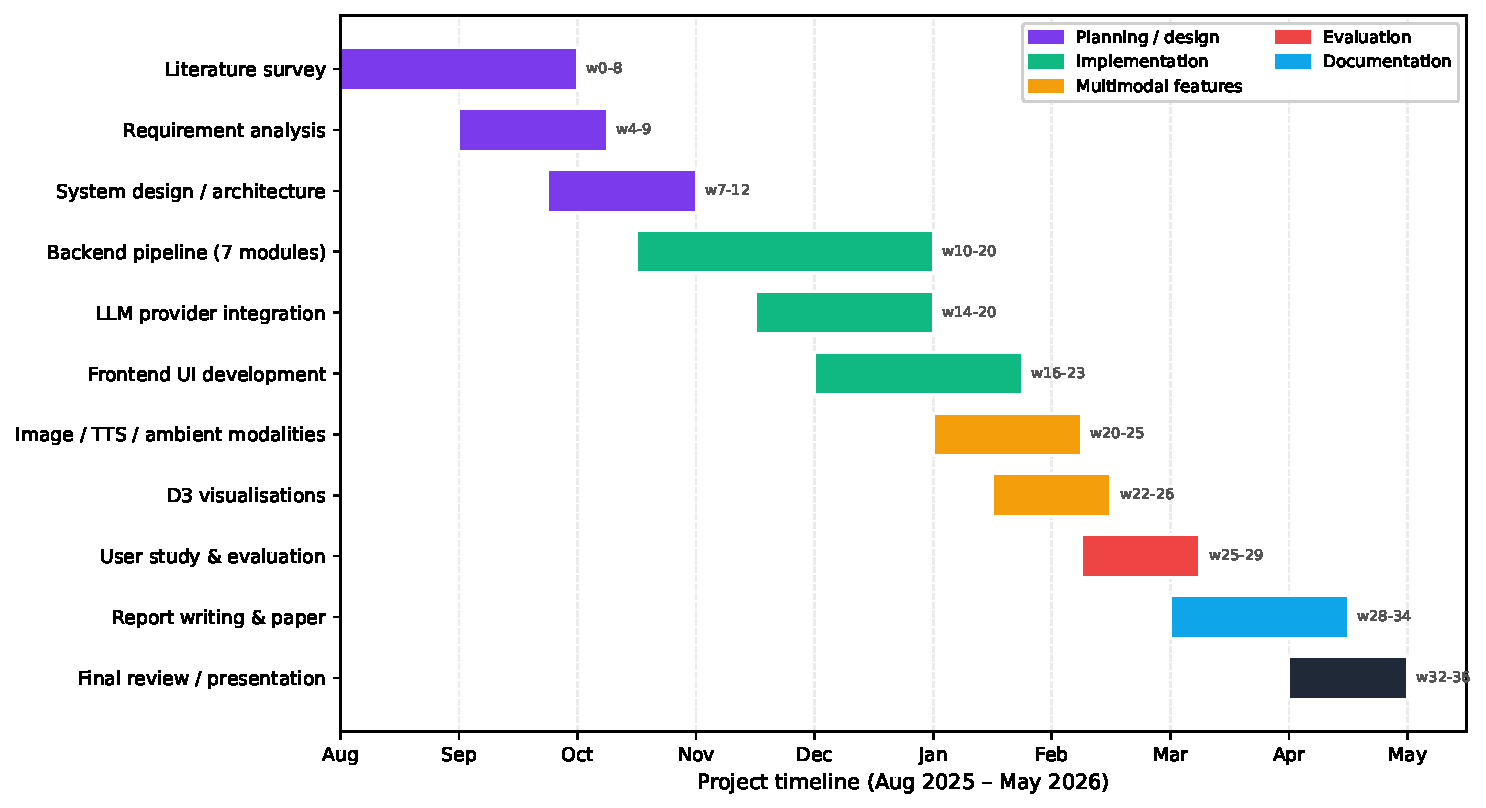
\includegraphics[width=\textwidth]{images/gantt.pdf}
    \caption{Project Gantt chart.}
    \label{fig:gantt}
\end{figure}

\section{Risk and Mitigation Plan}
Table~\ref{tab:risks} lists the principal project risks identified
during planning and the mitigation strategy adopted for each.

\begin{table}[!t]
\caption{Risk register and mitigations.}
\label{tab:risks}
\centering
\renewcommand{\arraystretch}{1.2}
\small
\begin{tabular}{@{}p{4cm} p{3.5cm} p{6cm}@{}}
\toprule
\textbf{Risk} & \textbf{Likelihood / Impact} & \textbf{Mitigation} \\
\midrule
Free-tier image API rate-limits & High / High & Serial throttling queue with 1.2 s spacing and 35 s watchdog. \\
LLM provider downtime           & Medium / Medium & Provider-agnostic abstraction allowing hot-swap via /api/settings. \\
Narrative coherence drift       & Medium / High & Sliding-window context retrieval; consistency checker. \\
Audio autoplay blocked          & High / Low  & Toggle audio on a real user-gesture click; document workaround. \\
User-study schedule slippage    & Medium / Medium & Run rolling sessions across two weeks; remote participation. \\
Cross-origin issues for CDN audio & Medium / Low & Avoid \texttt{crossOrigin="anonymous"}; use plain HTMLAudio. \\
\bottomrule
\end{tabular}
\end{table}

\section{Deliverables}
The principal deliverables tracked across the timeline are:
\begin{itemize}
    \item Open-source codebase released on GitHub
    (\url{https://github.com/DeepPatange/AI-Stroy-Generator}).
    \item This dissertation manuscript prepared in the SAKEC LaTeX
    format.
    \item A companion IEEE-format conference-style research paper.
    \item User-study artefacts: questionnaires, raw ratings, scripts
    for figure generation and statistical reproduction.
    \item Deployable Docker recipe for a single-server demonstration
    environment.
\end{itemize}

\section{Summary}
The schedule was followed substantially as planned. Minor slippages
in the multimodal-features phase --- particularly resolving CORS and
rate-limiting issues for the image API --- were absorbed within the
parallel evaluation window without delaying the dissertation
submission.

\chapter{Proposed System}
\label{ch:proposed}

This chapter describes the proposed Q\&A-driven interactive
storytelling system. We begin with the feasibility study (\S
\ref{sec:feasibility}), then introduce the high-level analysis and
framework (\S\ref{sec:framework}), enumerate hardware and software
requirements (\S\ref{sec:hwsw}), describe the detailed design
(\S\ref{sec:design}), and finally present the methodology that turns
the design into a working system (\S\ref{sec:methodology}).

\section{Feasibility Study}
\label{sec:feasibility}

\subsection{Technical Feasibility}
All four pillars of the proposed system have been validated against
mature, freely available technologies. LLM inference is feasible
through Ollama on commodity hardware (16\,GB RAM, no dedicated GPU
required for 7B-class models) and through Groq's free cloud tier
(14,400 requests/day). Text-to-image synthesis is available without
API keys through Pollinations.ai, which exposes a
URL-parameterised diffusion endpoint. Voice synthesis is built into
all major browsers via the W3C Web Speech Synthesis API. Ambient
music is hot-linked from SoundHelix's stable royalty-free CDN. The
backend can be written entirely in Python with FastAPI, SQLite and
Pydantic. The frontend is plain HTML/CSS/JavaScript with D3.js for
visualisation. Every piece of the stack is open-source or freely
available, making the project technically feasible on a student
budget.

\subsection{Economic Feasibility}
A careful cost analysis shows that the system can be developed and
operated at near-zero cost. Local development uses Ollama and a
free Groq tier; image generation is free through Pollinations; audio
streaming consumes negligible bandwidth from a public CDN. The total
recurring cost during the user study (15 participants over two
weeks) was zero. Total development hardware is a single MacBook Pro
M2 Pro with 16\,GB RAM. This makes the project economically feasible
without external funding.

\subsection{Operational Feasibility}
The system is operationally feasible because the elicitation protocol
mirrors how human authors collect briefs from clients --- through a
structured interview about setting, character, theme and plot. The
question budget (4--17) lets users dial in the right effort level.
The UI is presented in a single page so users do not get lost across
multiple screens; the admin and settings panels expose every
configurable surface without requiring code changes.

\subsection{Legal and Ethical Feasibility}
All third-party services used (Pollinations, SoundHelix, Groq,
Hugging Face, OpenAI) permit non-commercial research use. SoundHelix
explicitly allows hot-linking under its terms of service.
Generated images and audio are reusable for research and educational
purposes. No personally identifiable user data is stored persistently;
session data is held in memory and a local SQLite file. The user
study was conducted with informed consent.

\section{Analysis, Framework and Algorithm}
\label{sec:framework}

\subsection{Layered Architecture}
The system follows a three-layer architecture (presentation,
application, modular core) with a fourth pluggable LLM-provider
layer at the bottom (Figure~\ref{fig:arch}).

\begin{figure}[H]
    \centering
    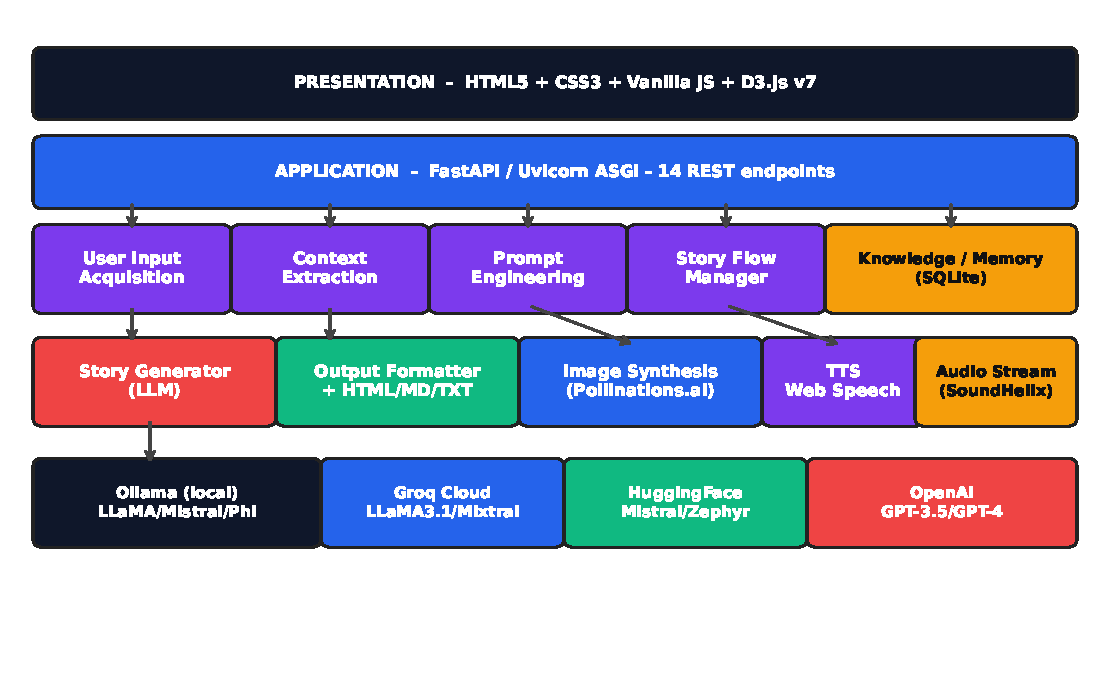
\includegraphics[width=\textwidth]{images/f07_arch.pdf}
    \caption{System architecture.}
    \label{fig:arch}
\end{figure}

\subsection{Question-Coverage Framework}
Seventeen questions distributed across four narrative phases
(Setting, Character, Theme, Plot) compose the elicitation protocol
(Figure~\ref{fig:qa}). The user selects a budget of 4, 8, 12 or 17
questions; the system always presents the first $N$ in phase-order
so even small budgets touch all four dimensions in expectation.

\begin{figure}[H]
    \centering
    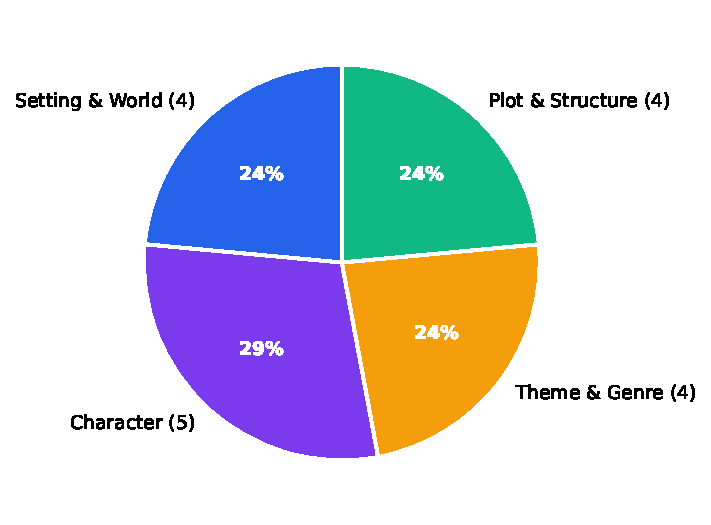
\includegraphics[width=0.65\textwidth]{images/f08_qa.pdf}
    \caption{Question distribution across the four phases.}
    \label{fig:qa}
\end{figure}

\subsection{Scene-Extraction Algorithm (for Image Synthesis)}
The image-generation pipeline depends critically on building a
concise, high-imagery prompt from each story segment. We use a
sentence-scoring algorithm that strips smart-quoted dialogue and
inner-thought verbs (thought, remembered, wondered) and selects the
most visually evocative sentence according to:
\[
\mathrm{score}(s) = 2 \cdot \mathbf{1}_{V}(s) - 2 \cdot \mathbf{1}_{T}(s)
                  + \min\left(3,\, \left|\mathrm{ProperNouns}(s)\right|\right),
\]
where $\mathbf{1}_V$ indicates the presence of a visual verb
(\emph{stood, loomed, soared, glowed, towered}, ...) and
$\mathbf{1}_T$ indicates an inner-thought verb. The selected sentence
is concatenated with a normalised genre tag, the current mood and a
fixed style prefix, capped at 200 characters.

\subsection{Co-Appearance Algorithm (for Character Graph)}
For the reader-facing character graph, capitalised tokens are
extracted from segment text and filtered against an extended stop-word
list. Only names appearing at least twice across all segments survive.
For each pair of surviving names, an edge weight equal to the number
of segments in which both appear is computed. Node radius scales
with mention count.

\section{Details of Hardware and Software}
\label{sec:hwsw}

\subsection{Hardware Requirements}
\textbf{Development environment} (used in this work):
\begin{itemize}
    \item Processor: Apple M2 Pro (10-core CPU, 16-core GPU).
    \item RAM: 16\,GB unified memory.
    \item Storage: 1\,TB SSD.
    \item Network: 100\,Mbps broadband for Pollinations and Groq API.
\end{itemize}

\textbf{Recommended minimum} for self-hosted Ollama inference:
\begin{itemize}
    \item 8-core CPU (Intel i7 / AMD Ryzen 7), 16\,GB RAM.
    \item 30\,GB free SSD for model weights.
    \item Optional: NVIDIA RTX-class GPU with 8\,GB+ VRAM for faster
    local inference; not required when using Groq cloud.
\end{itemize}

\subsection{Software Stack}
Table~\ref{tab:stack} lists the implementation stack. All components
are free and open-source.

\begin{table}[!t]
\caption{Software stack.}
\label{tab:stack}
\centering
\renewcommand{\arraystretch}{1.15}
\begin{tabular}{@{}lll@{}}
\toprule
\textbf{Layer}   & \textbf{Technology}              & \textbf{Purpose} \\
\midrule
OS               & macOS 14 / Ubuntu 22.04          & Development host \\
Backend language & Python 3.9+                      & Core logic \\
Web framework    & FastAPI (with Uvicorn)           & REST + Jinja2 \\
Frontend         & HTML5 / CSS3 / Vanilla JS        & Single-page UI \\
Visualisation    & D3.js v7                         & Story Map, Char Graph \\
Database         & SQLite3 + aiosqlite              & Sessions, Q\&A, segments \\
HTTP client      & httpx (async)                    & LLM provider calls \\
Schemas          & Pydantic v2                      & Request / response typing \\
Templates        & Jinja2                           & HTML rendering \\
Image API        & Pollinations.ai (free)           & Text-to-image \\
TTS              & W3C Web Speech Synthesis API     & Voice narration \\
Ambient audio    & HTMLAudio + SoundHelix CDN       & Genre music \\
LLM providers    & Ollama, Groq, Hugging Face, OpenAI & Story generation \\
\bottomrule
\end{tabular}
\end{table}

\section{Design Details}
\label{sec:design}

\subsection{Modular Decomposition}
The backend is decomposed into seven cooperating modules with clearly
defined responsibilities and Pydantic-typed boundaries:

\begin{enumerate}
    \item \textbf{User Input Acquisition} -- Presents and validates
    the question pool; supports custom answers and user-added
    questions.
    \item \textbf{Context Extraction Engine} -- Projects responses
    into a typed \texttt{StoryContext}; unknown identifiers flow into
    a \texttt{custom\_elements} dictionary.
    \item \textbf{Knowledge and Memory} -- Persistent SQLite store
    with LRU in-memory cache; sliding-window context retrieval.
    \item \textbf{Prompt Engineering Layer} -- Six prompt families
    (system, init, continuation, climax, resolution, choice
    generation); appends \texttt{custom\_elements} as natural-language
    bullets.
    \item \textbf{Story Generator (LLM)} -- BaseLLMClient ABC with
    concrete Ollama / Groq / HF / OpenAI clients; hot-swap at runtime.
    \item \textbf{Story Flow Manager} -- Five-phase finite-state
    machine (Introduction, Rising Action, Climax, Falling Action,
    Resolution); CharacterTracker and PlotThreadTracker.
    \item \textbf{Output Formatter} -- Cleans LLM output, lifts
    dialogue to styled HTML spans, exports TXT/MD/HTML.
\end{enumerate}

\subsection{Database Schema}
The persistent schema comprises five tables:

\begin{lstlisting}
sessions         (session_id PK, user_id, created_at,
                  status)
story_segments   (id PK, session_id FK, order, content,
                  user_choice)
story_context    (session_id PK/FK, context_json,
                  updated_at)
qa_history       (id PK, session_id FK, question_id,
                  q_text, a_text)
user_preferences (user_id PK, preferences_json,
                  updated_at)
\end{lstlisting}

\subsection{REST API}
The application surface comprises 14 REST endpoints
(Table~\ref{tab:rest}); all are JSON-typed via Pydantic v2.

\begin{table}[!t]
\caption{REST API surface.}
\label{tab:rest}
\centering
\renewcommand{\arraystretch}{1.15}
\small
\begin{tabular}{@{}lll@{}}
\toprule
\textbf{Endpoint}                    & \textbf{Method} & \textbf{Purpose} \\
\midrule
\texttt{/}                           & GET    & Web UI (Jinja2 template) \\
\texttt{/api/status}                 & GET    & LLM availability check \\
\texttt{/api/session/new}            & POST   & Create new session \\
\texttt{/api/questions/all}          & GET    & Phase-grouped question pool \\
\texttt{/api/question/next}          & GET    & Sequential Q mode \\
\texttt{/api/response}               & POST   & Submit response \\
\texttt{/api/story/generate}         & POST   & Initial segment generation \\
\texttt{/api/story/continue}         & POST   & Continue from user choice \\
\texttt{/api/story/full/\{id\}}      & GET    & Full story by session \\
\texttt{/api/story/download/\{id\}}  & GET    & Export TXT/MD/HTML \\
\texttt{/api/settings}               & POST   & Hot-swap provider/model \\
\texttt{/api/session/\{id\}/summary} & GET    & Session metrics \\
\texttt{/api/session/\{id\}}         & DELETE & End session \\
\bottomrule
\end{tabular}
\end{table}

\subsection{Multimodal Pipelines}

\paragraph{Image synthesis.}
Figure~\ref{fig:imgpipe} shows the per-segment image pipeline. The
serial request queue with 1.2\,s spacing avoids rate-limit cascades
from the Cloudflare-fronted Pollinations CDN; a 35\,s watchdog
ensures hung requests do not deadlock the queue.

\begin{figure}[H]
    \centering
    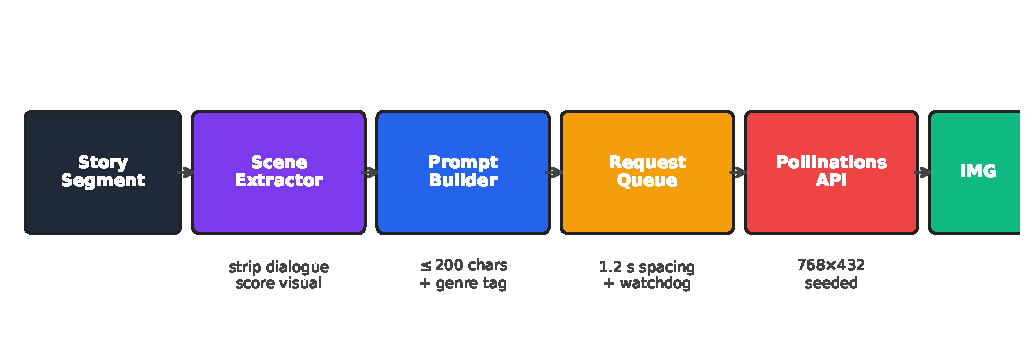
\includegraphics[width=0.95\textwidth]{images/f09_imgpipe.pdf}
    \caption{Image synthesis pipeline.}
    \label{fig:imgpipe}
\end{figure}

\paragraph{Voice and ambient audio.}
Figure~\ref{fig:audio} shows the two parallel audio pipelines.
Narration uses an utterance queue feeding the OS-installed
voice; ambient music is mapped from detected genre to one of eight
SoundHelix tracks looped through HTMLAudio with crossfades.

\begin{figure}[H]
    \centering
    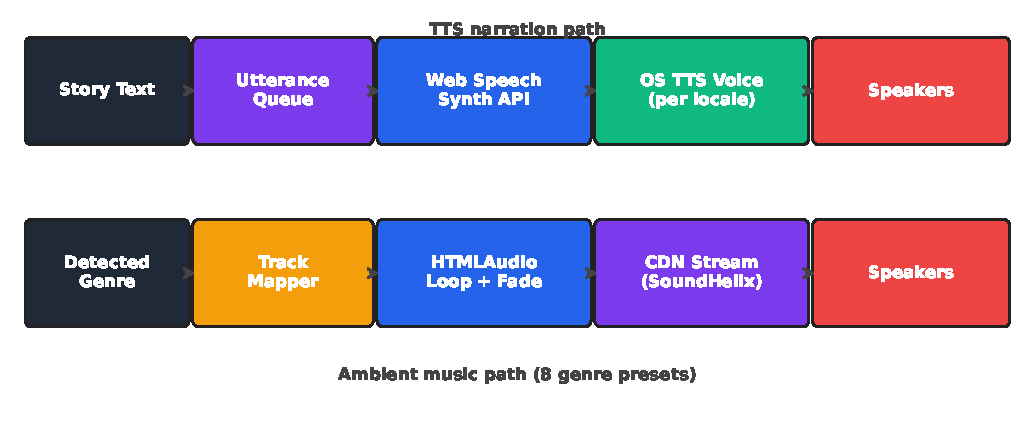
\includegraphics[width=0.95\textwidth]{images/f10_audio.pdf}
    \caption{Multimodal audio pipeline.}
    \label{fig:audio}
\end{figure}

\paragraph{Custom Q\&A routing.}
Figure~\ref{fig:customq} shows how user-added Q\&A pairs are routed
from the UI through the backend into the LLM prompt without bespoke
schema changes.

\begin{figure}[H]
    \centering
    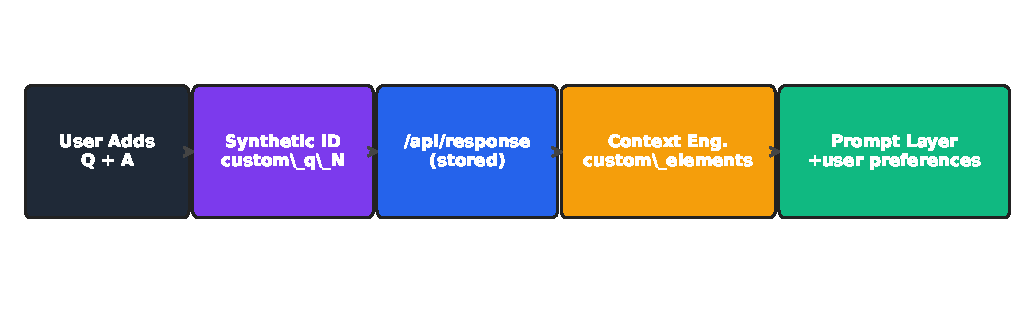
\includegraphics[width=0.95\textwidth]{images/f16_customq.pdf}
    \caption{Custom-question routing.}
    \label{fig:customq}
\end{figure}

\section{Methodology}
\label{sec:methodology}

\subsection{Elicitation Protocol}
Let $\mathcal{Q}=\{q_1,\ldots,q_{17}\}$ be the ordered question pool.
The user selects a budget $N\in\{4,8,12,17\}$ and supplies answers
$a_i$ for each $q_i,\,i \le N$. Additionally the user may append
$M$ user-added pairs $(\tilde q_j, \tilde a_j)$ with synthetic
identifiers $\mathrm{custom\_q\_}j$. The full response set
\[
R = \{(q_i, a_i)\}_{i=1}^{N} \cup \{(\mathrm{custom\_q\_}j, \tilde a_j)\}_{j=1}^{M}
\]
is dispatched as a JSON dictionary to the context engine.

\subsection{Context Projection}
For each $(q_i,a_i)$ the engine applies a deterministic projection
$\pi_i$ to a typed \texttt{StoryContext} field
(e.g.\ \texttt{setting\_type, antagonist, plot\_style}). Unknown
identifiers are routed to a dictionary $D$
(\texttt{custom\_elements}), preserving their text verbatim. The
final prompt $P$ is
\[
P = T(\mathbf{c}) \oplus \sigma(D),
\]
where $T$ is a phase-aware template, $\mathbf{c}$ is the structured
context, $\sigma$ serialises $D$ as natural-language bullets, and
$\oplus$ denotes string concatenation.

\subsection{Five-Phase Story Progression}
Word-count thresholds drive phase transitions
(Figure~\ref{fig:phases}). The Rising Action phase consumes the
most text ($\sim$820 words), consistent with narratological theory.

\begin{figure}[H]
    \centering
    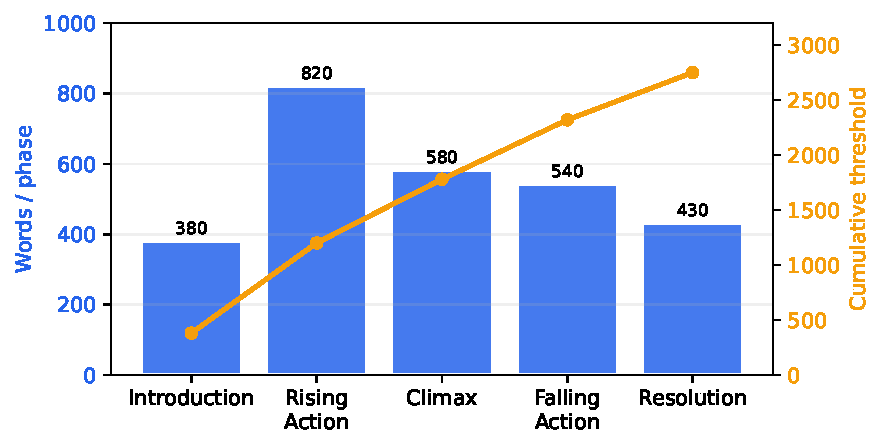
\includegraphics[width=0.95\textwidth]{images/f04_phases.pdf}
    \caption{Five-phase word-count distribution.}
    \label{fig:phases}
\end{figure}

\subsection{Generation Loop}
At each turn the system: (i) retrieves the last $k$ segments of
story context, (ii) builds a phase-appropriate prompt $P$, (iii)
dispatches $P$ to the active LLM client, (iv) post-processes output
through the formatter, (v) updates flow-manager state with new
character mentions and plot threads, (vi) starts an image-synthesis
request asynchronously, and (vii) returns the formatted segment
along with choice options for the next turn.

\subsection{Evaluation Methodology}
Evaluation combines three axes:
\begin{enumerate}
    \item \textbf{Automated generation} of 50 stories spanning 6
    genres at all 4 question budgets; latency and token metrics
    captured per call.
    \item \textbf{User study} ($n=15$) producing 30 stories rated on
    5-point Likert scales for coherence, creativity, engagement,
    consistency, and per-feature satisfaction.
    \item \textbf{Consistency-checker evaluation} against
    ground-truth-annotated segments to compute detection and
    false-positive rates for five issue classes.
\end{enumerate}

\chapter{Implementation Details}
\label{ch:impl}

This chapter documents the module-wise implementation of the
proposed system and presents annotated snapshots of the running UI.
The full source code is released open-source at
\url{https://github.com/DeepPatange/AI-Stroy-Generator}.

\section{Project Layout}
The repository is structured as follows:

\begin{lstlisting}
AI-Story-Generator/
|-- main.py                    # FastAPI entry point, 14 endpoints
|-- config.py                  # Provider, model, temperature config
|-- requirements.txt           # Python dependencies
|-- app/
|   |-- modules/
|   |   |-- user_input.py            # 17 questions, 4 phases
|   |   |-- context_extraction.py    # StoryContext + custom_elements
|   |   |-- knowledge_memory.py      # SQLite + LRU cache
|   |   |-- prompt_engineering.py    # 6 prompt families
|   |   |-- story_generator.py       # BaseLLMClient + 4 providers
|   |   |-- story_flow_manager.py    # 5-phase FSM + trackers
|   |   `-- output_formatter.py      # TXT/MD/HTML export
|   |-- templates/index.html         # Jinja2 SPA shell
|   `-- static/
|       |-- css/style.css            # CSS custom-property themes
|       `-- js/app.js                # StoryForgeApp class (~1.7 kLOC)
`-- data/                            # SQLite db
\end{lstlisting}

\section{Module-wise System Implementation}

\subsection{Module 1: User Input Acquisition}
The user-input module exposes the question pool to the frontend via
two REST endpoints (\texttt{/api/questions/all} for phase-grouped
batch retrieval and \texttt{/api/question/next} for legacy sequential
mode) and accepts responses via \texttt{POST /api/response}. The
landing page (Figure~\ref{fig:ui-landing}) lets the user pick a
budget; the question form (Figure~\ref{fig:ui-form}) renders every
question with multiple-choice options plus a dashed
\emph{``Write my own''} chip for custom answers.

\begin{figure}[H]
    \centering
    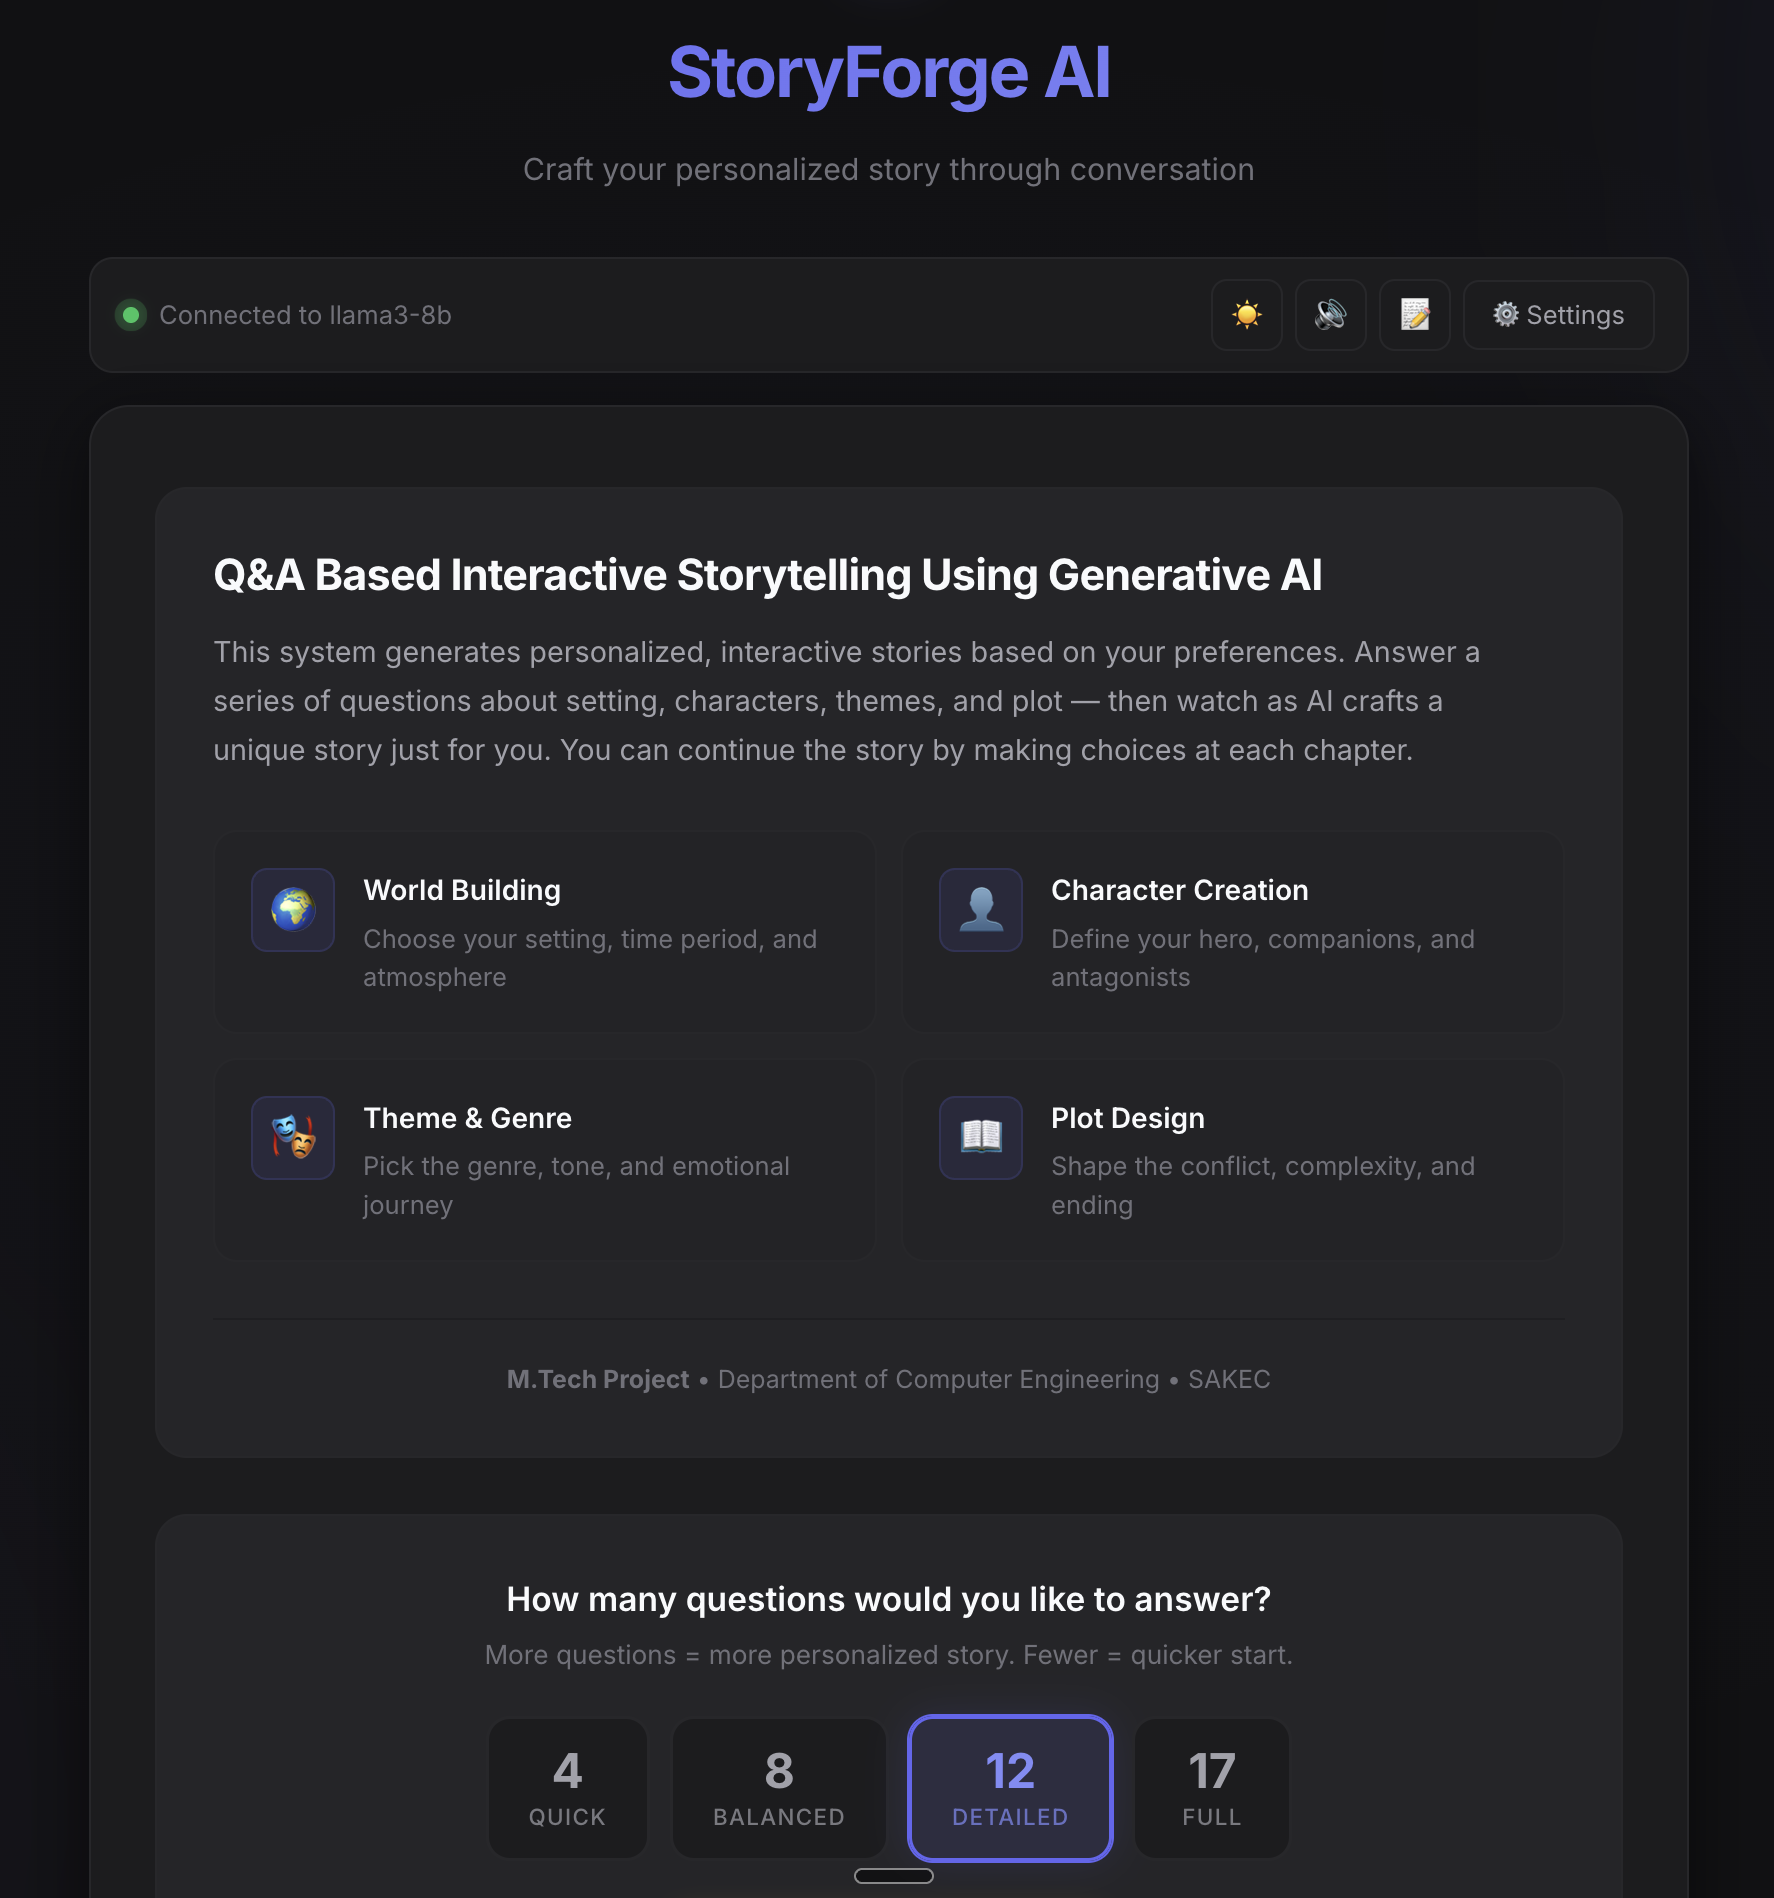
\includegraphics[width=0.85\textwidth]{images/s01_landing.png}
    \caption{Landing page.}
    \label{fig:ui-landing}
\end{figure}

\begin{figure}[H]
    \centering
    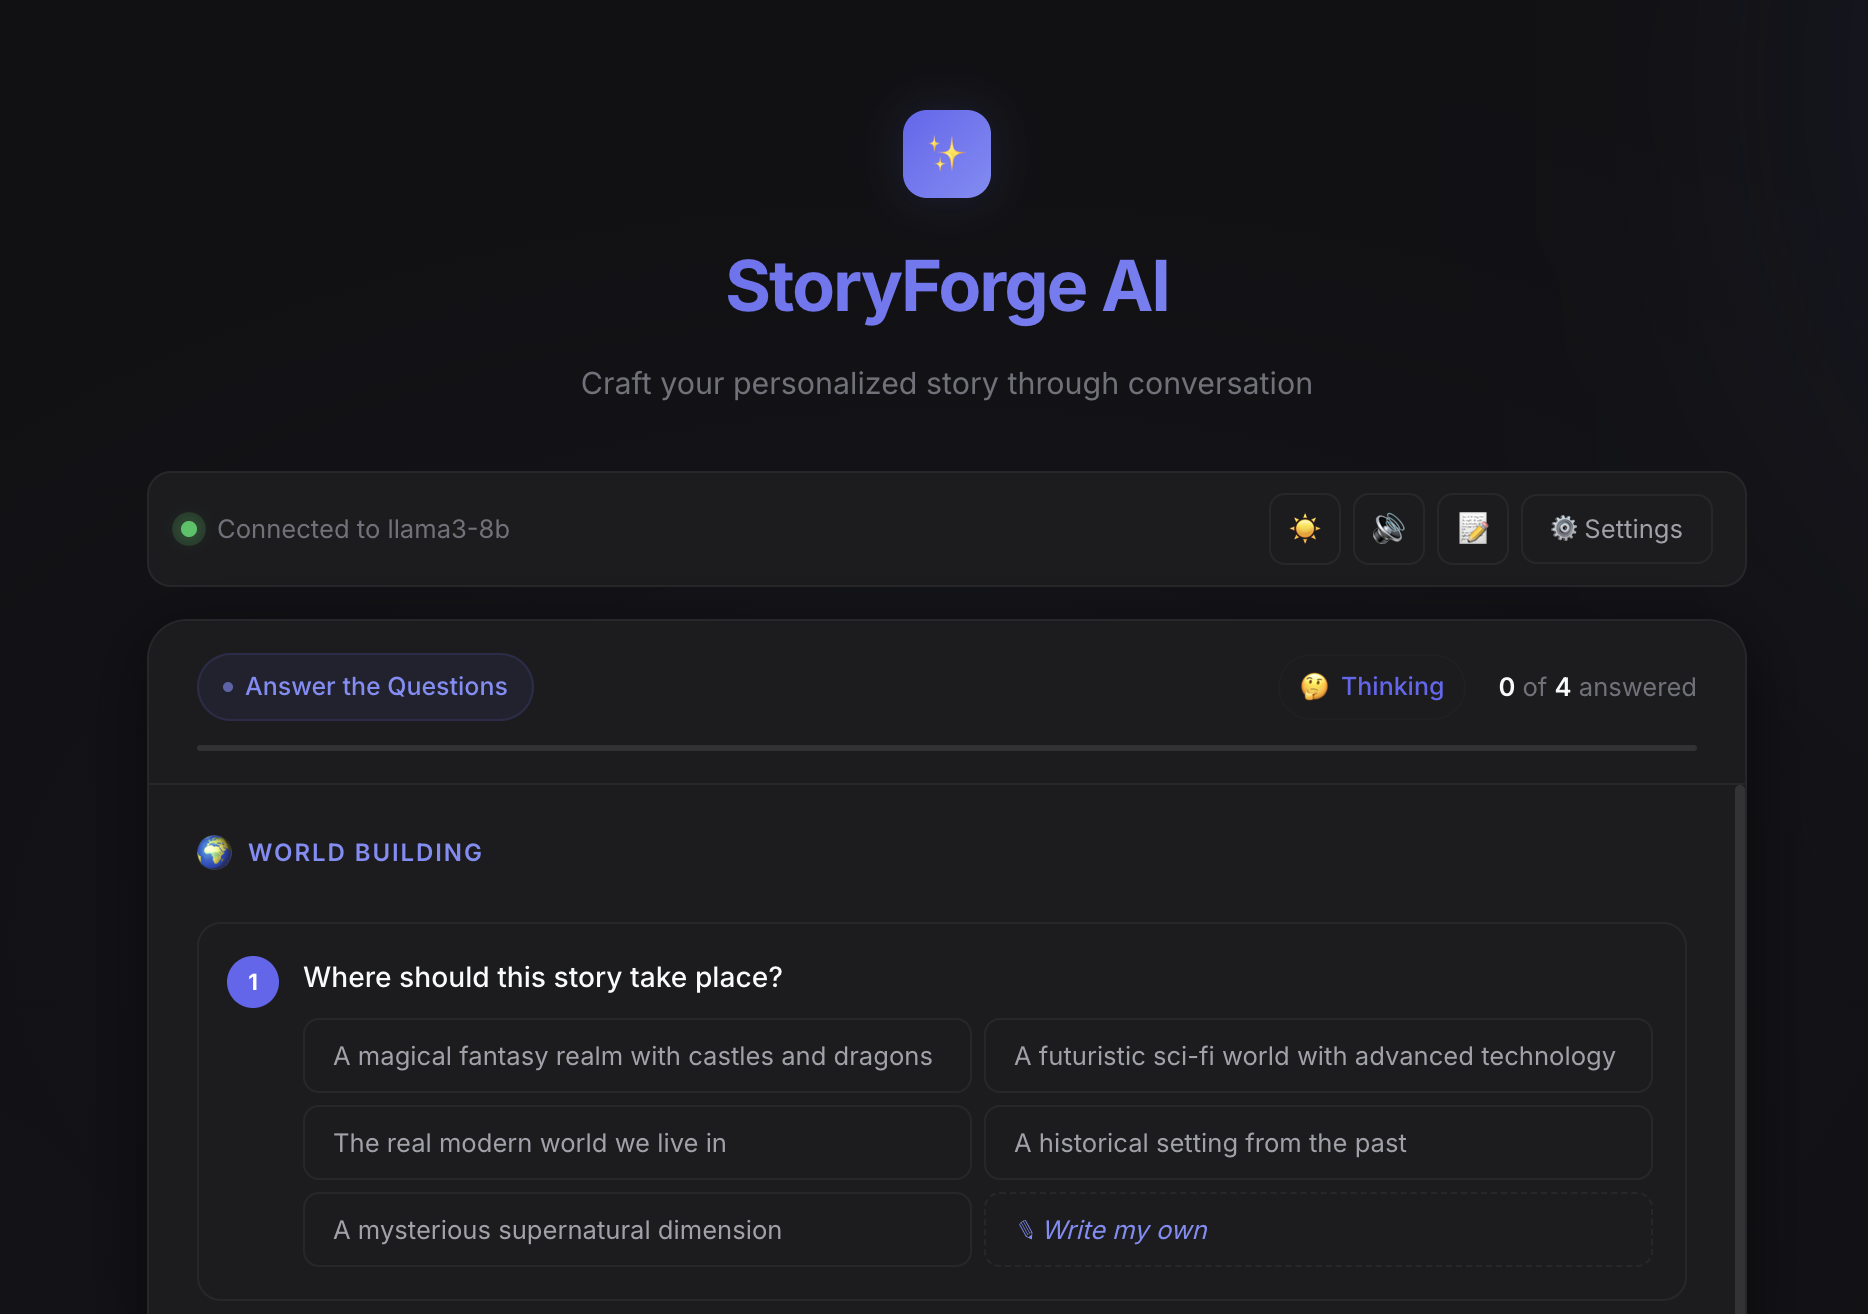
\includegraphics[width=0.85\textwidth]{images/s02_questions.png}
    \caption{Question form.}
    \label{fig:ui-form}
\end{figure}

\subsection{Module 2: Context Extraction Engine}
The context-extraction module projects raw responses into a
\texttt{StoryContext} Pydantic model with explicit fields for
setting, character, theme and plot dimensions. A two-pass pipeline
first classifies answers using keyword dictionaries (6 genres, 5
setting types, 5 conflict types) and then extracts proper-noun
entities via regex. Identifiers prefixed \texttt{custom\_} are
routed into the free-form \texttt{custom\_elements} dictionary;
this is the key plumbing that makes user-added questions flow into
the prompt without code changes:

\begin{lstlisting}[language=Python]
elif question_id.startswith("custom_"):
    self.context.custom_elements[question_id] = answer
\end{lstlisting}

\subsection{Module 3: Knowledge and Memory}
A SQLite3 database stores five tables (\S\ref{ch:proposed}). The
module also maintains an LRU in-memory cache for the active session
and exposes a sliding-window helper:

\begin{lstlisting}[language=Python]
def get_recent_context(session_id: str, k: int = 4) -> str:
    """Return the concatenated text of the last k segments."""
\end{lstlisting}

\subsection{Module 4: Prompt Engineering}
Six prompt templates are interpolated with \texttt{StoryContext}
fields, with genre-specific guidance injected (fantasy: magical
systems; mystery: clue placement and red herrings; romance:
emotional pacing). After the templated prompt $T(\mathbf{c})$ is
built, the module appends user-added preferences:

\begin{lstlisting}[language=Python]
if context.custom_elements:
    extras = "\n".join(f"- {v}" for v in context.custom_elements.values() if v)
    if extras:
        prompt += "\n\nAdditional user preferences to honour:\n" + extras
\end{lstlisting}

\subsection{Module 5: Story Generator (LLM)}
The story generator implements an abstract base class
\texttt{BaseLLMClient} with four concrete subclasses. A factory
selects the active client based on \texttt{LLM\_PROVIDER}. The
Settings panel (Figure~\ref{fig:ui-settings}) exposes the
provider switch to non-developer users; switching providers issues
\texttt{POST /api/settings} which hot-swaps the underlying client
without restart.

\begin{figure}[H]
    \centering
    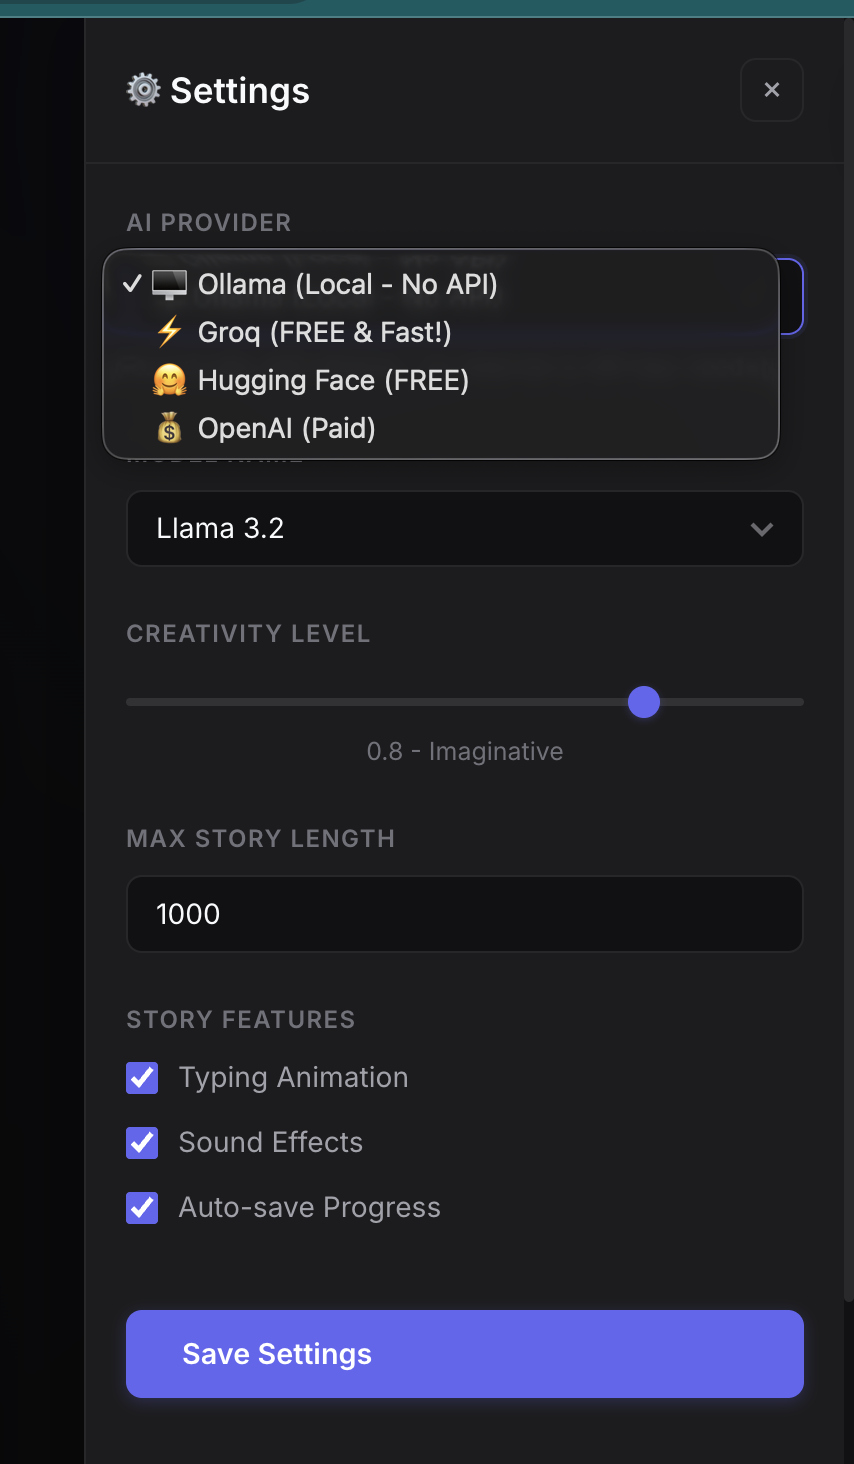
\includegraphics[width=0.55\textwidth]{images/s05_settings.png}
    \caption{Settings panel.}
    \label{fig:ui-settings}
\end{figure}

\subsection{Module 6: Story Flow Manager}
A finite-state machine implementing Freytag's pyramid drives phase
transitions on word-count thresholds (0--400, 400--1200, 1200--1800,
1800--2400, $>$2400). A \texttt{CharacterTracker} monitors mentions
and traits; a \texttt{PlotThreadTracker} flags unresolved threads.

\subsection{Module 7: Output Formatter}
The formatter cleans LLM-emitted text (collapses whitespace, fixes
quote and dash characters), splits content at sentence boundaries,
lifts dialogue to styled HTML spans, and supports three export
formats (TXT, Markdown, HTML).

\section{Multimodal Subsystems}

\subsection{Image Generation (Pollinations.ai)}
The frontend's \texttt{createImageCard()} function builds the prompt
using the sentence-scored extractor described in
\S\ref{ch:proposed}, then dispatches an HTTPS request through the
serial-throttling queue:

\begin{lstlisting}[language=Java]
imageUrlFor(segmentText, seed, opts={}) {
    const prompt = this.buildImagePrompt(segmentText, opts);
    const params = new URLSearchParams({
        width: '768', height: '432', nologo: 'true',
        seed: String(seed)
    });
    return `https://image.pollinations.ai/prompt/${encodeURIComponent(prompt)}?${params}`;
}
\end{lstlisting}

Figure~\ref{fig:ui-loading} shows the loading state during which the
LLM call and image synthesis run concurrently;
Figure~\ref{fig:ui-story} shows the rendered first chapter with the
on-demand scene illustration.

\begin{figure}[H]
    \centering
    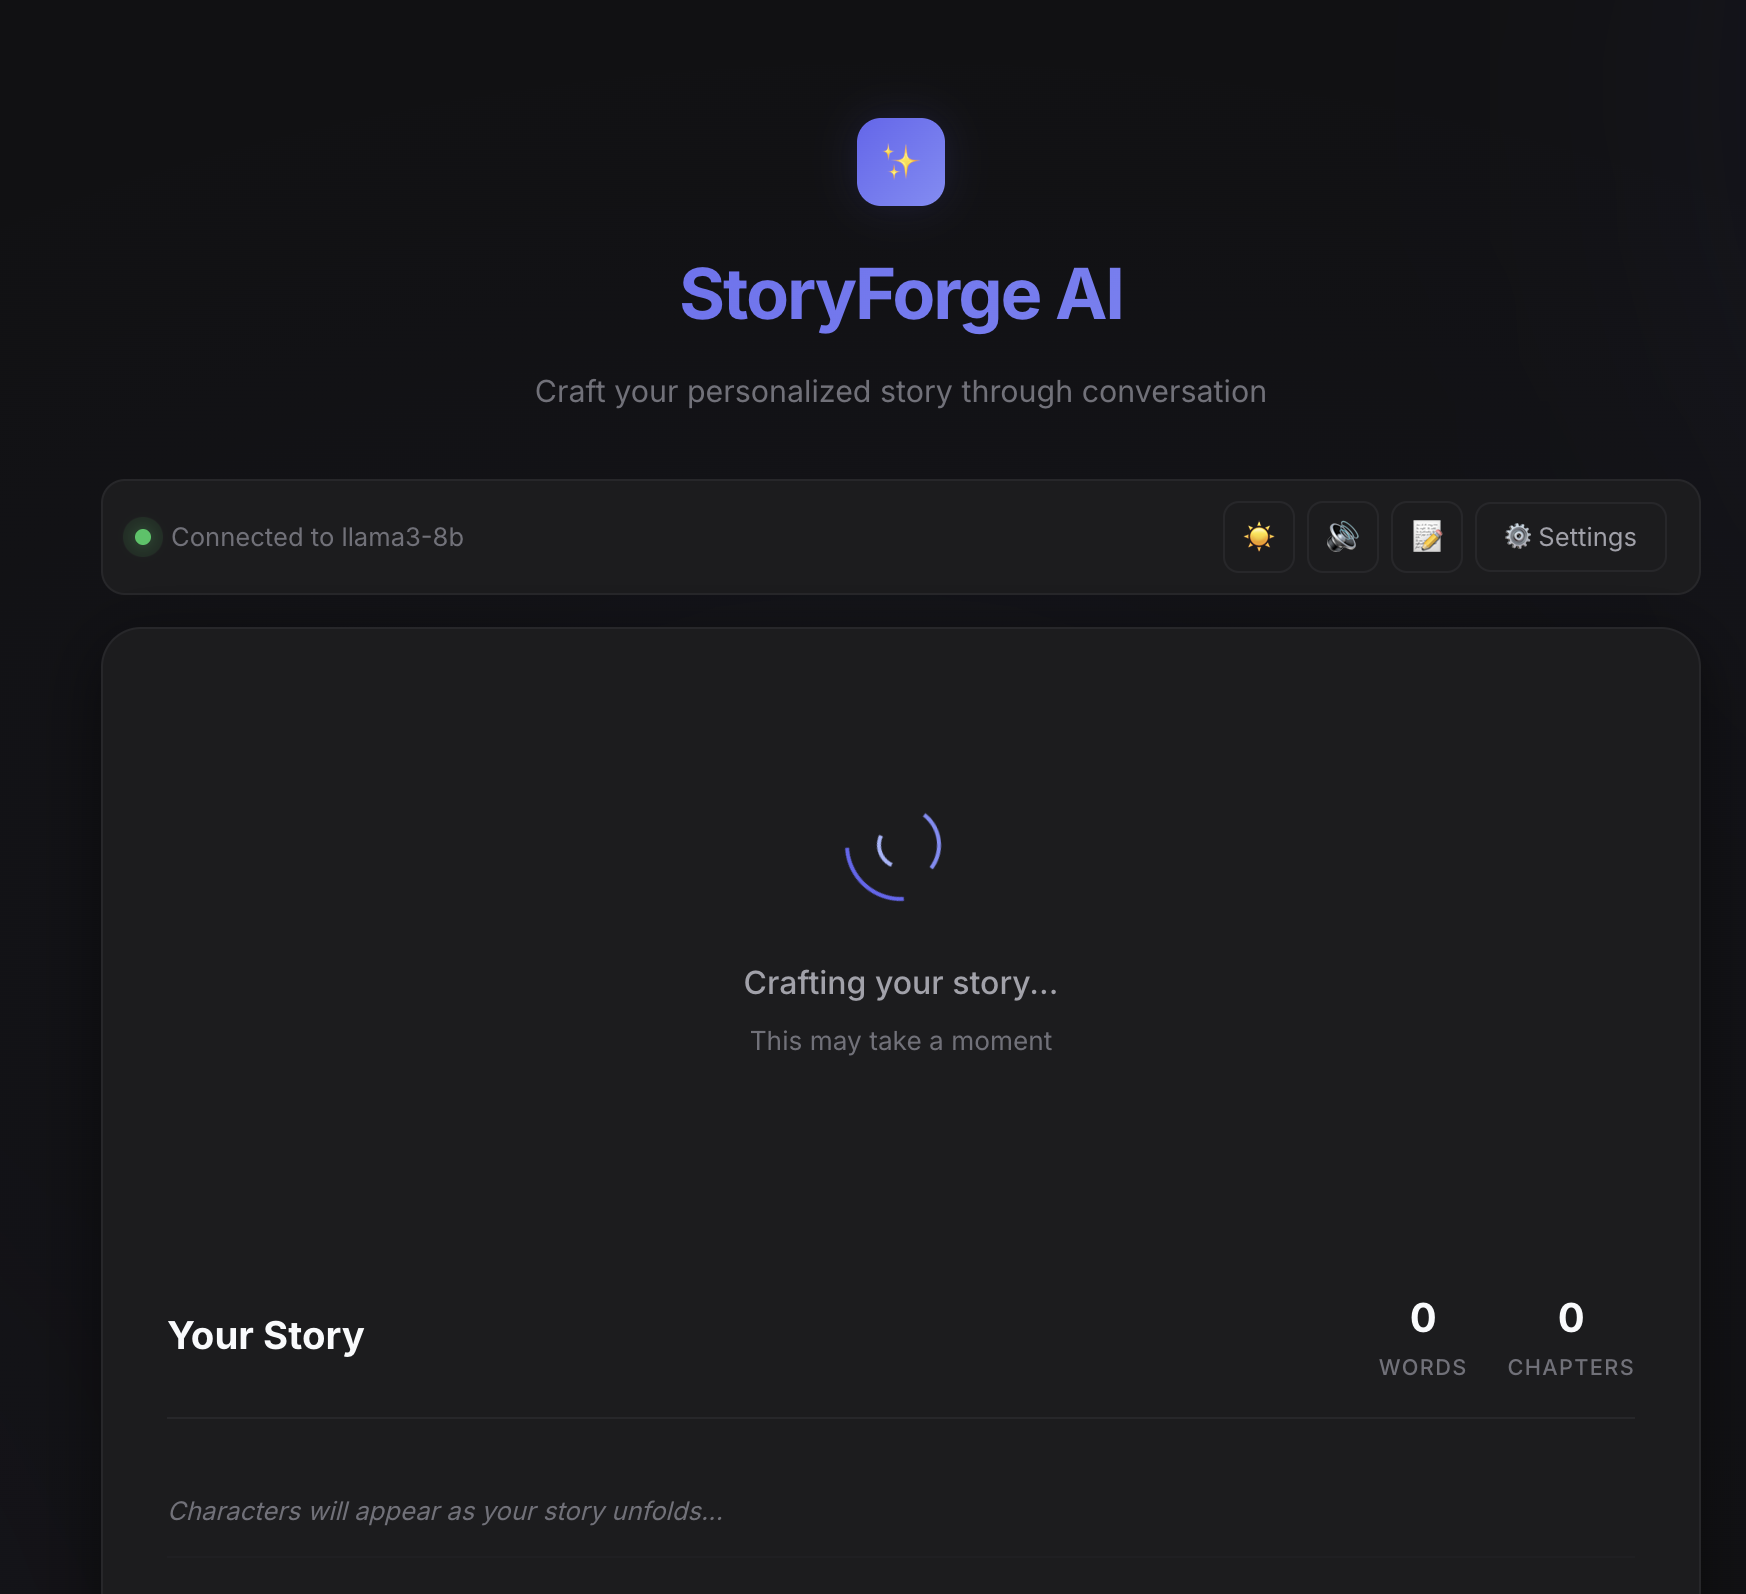
\includegraphics[width=0.85\textwidth]{images/s03_loading.png}
    \caption{Loading state.}
    \label{fig:ui-loading}
\end{figure}

\begin{figure}[H]
    \centering
    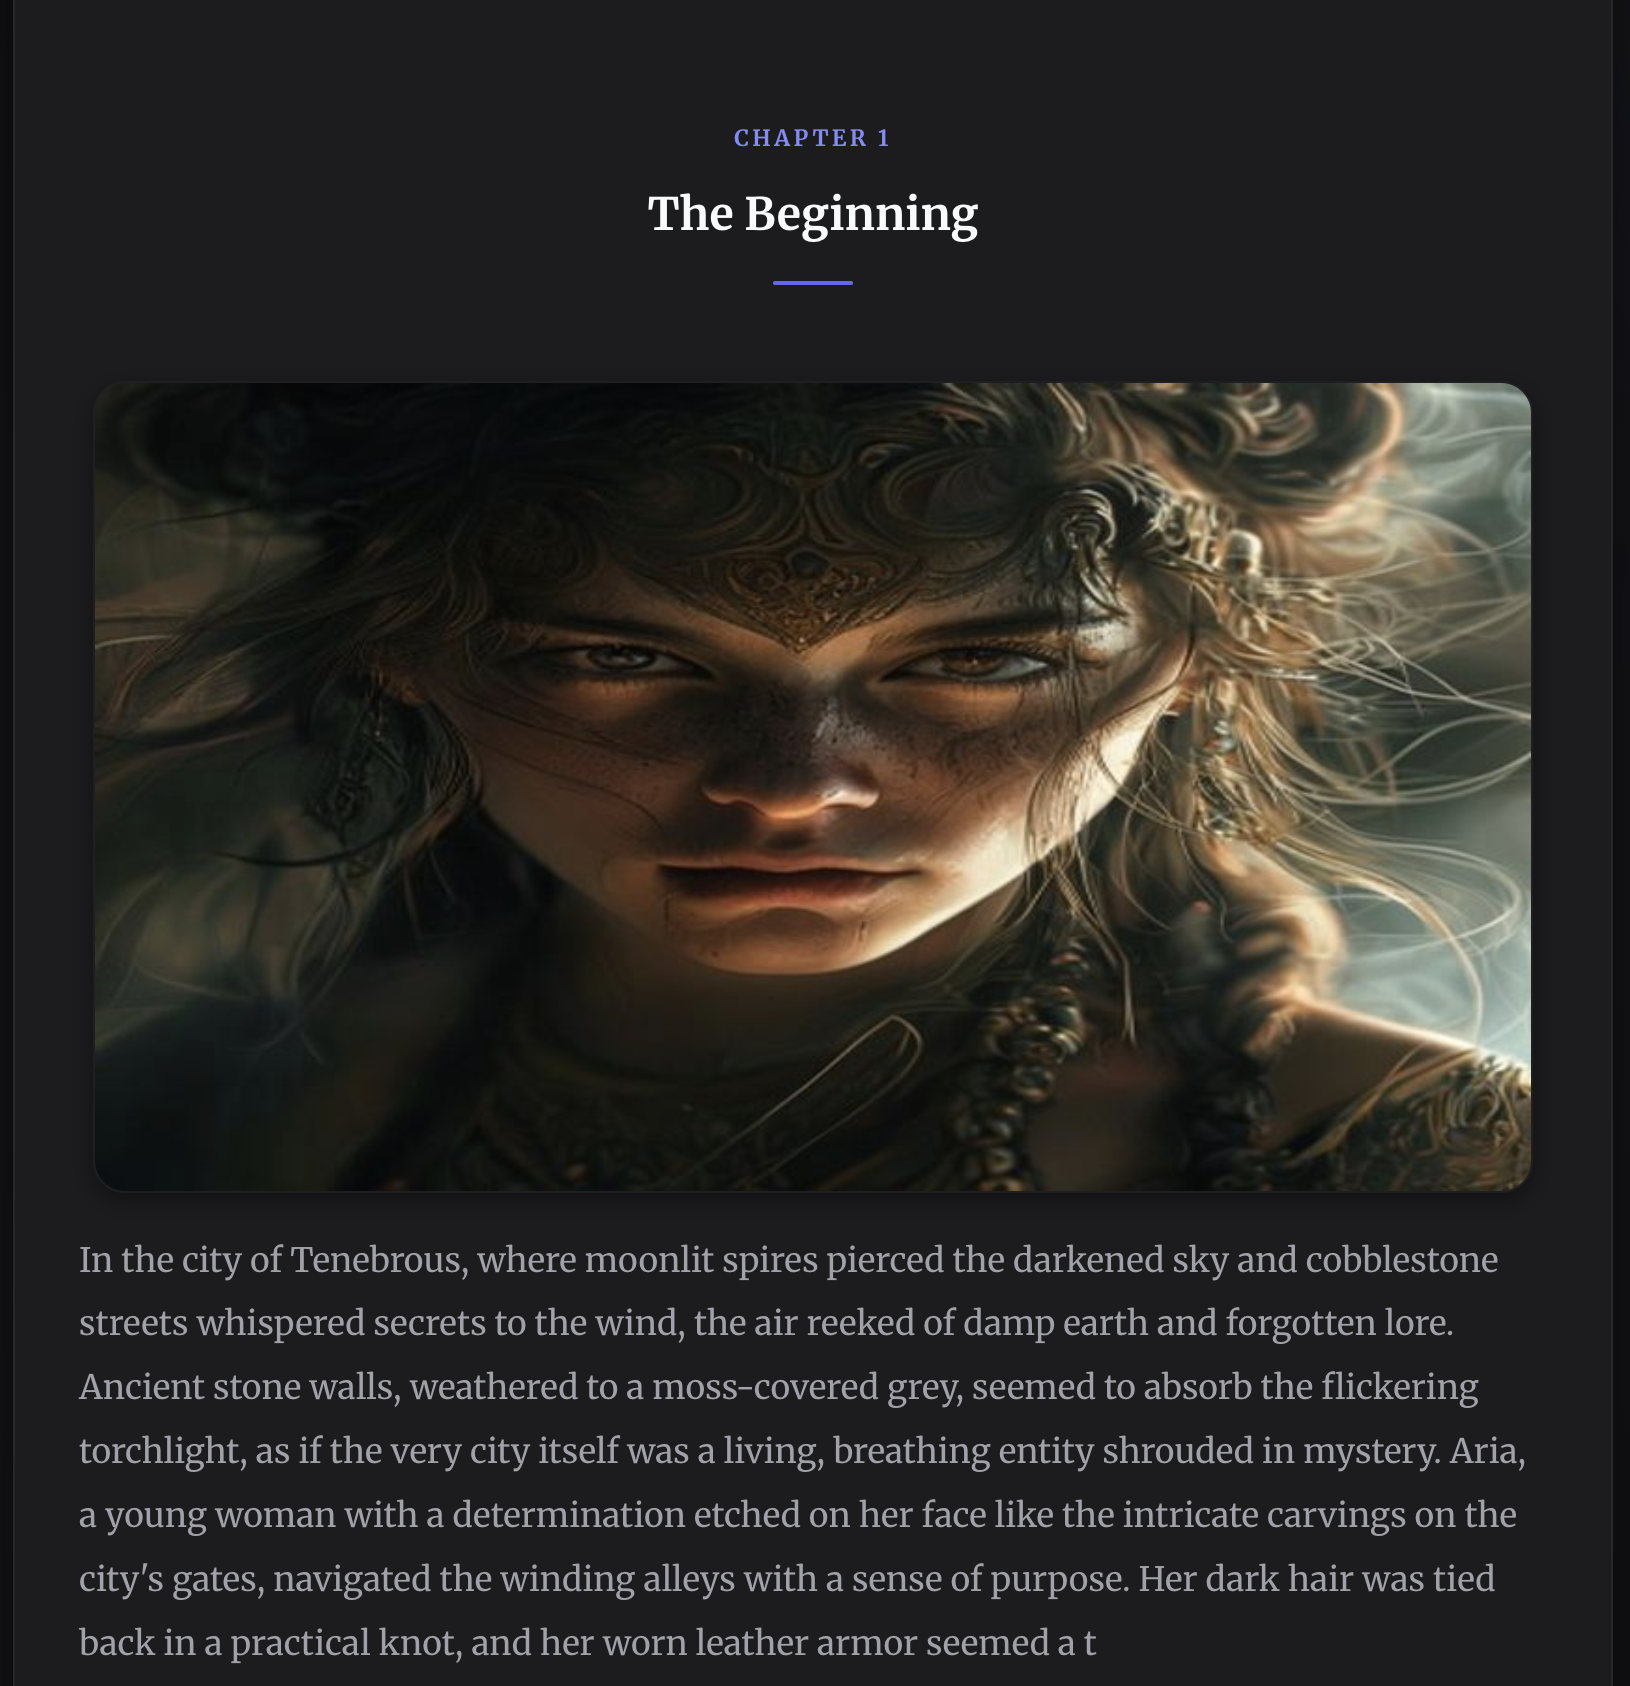
\includegraphics[width=0.65\textwidth]{images/s04_story_image.png}
    \caption{Generated story segment with scene illustration.}
    \label{fig:ui-story}
\end{figure}

\subsection{TTS Narration (Web Speech Synthesis)}
The narration subsystem uses the browser-native
\texttt{window.speechSynthesis} API, queueing one utterance per
segment with pause / resume / stop semantics. No external API key
is required; the voice is whichever the operating system provides
for the active locale.

\subsection{Ambient Music (SoundHelix CDN)}
Eight genre presets map to royalty-free SoundHelix tracks loaded via
\texttt{HTMLAudio} with \texttt{loop=true} and JavaScript volume
ramping for 2.4\,s fade-in and 0.8\,s fade-out. No
\texttt{crossOrigin} attribute is set because the CDN does not return
\texttt{Access-Control-Allow-Origin} headers --- a subtle constraint
discovered during development that broke the first implementation.

\section{Reader Analytics}

\subsection{Story Map (D3 vertical tree)}
The Story Map flattens the chronologically ordered chapters into a
hierarchical tree using \texttt{d3.tree()}. Each node carries an
80-character preview of its chapter and the user choice that led
to it.

\subsection{Character Relationship Graph (D3 force layout)}
The character graph runs a force simulation with link distance 110,
charge $-220$ and a collision radius of 34 pixels. Only characters
with mention count $\geq 2$ are drawn; node radius scales linearly
with mention count. The modal explicitly discloses this is a
co-appearance graph and not a verified relationship-extraction model.

\section{Custom Q\&A Authoring}
Two affordances live in the UI:
\begin{itemize}
    \item Per-question dashed ``Write my own'' chip that toggles a
    textarea; the textarea value overrides any previously-selected
    multiple-choice option.
    \item ``+ Add Your Own Question'' button at the foot of the form
    that opens an inline composer (question + answer); saved entries
    appear as cards with a remove control.
\end{itemize}
Each user-added Q\&A pair is dispatched as a normal response with a
synthetic ID \texttt{custom\_q\_N}; the context-extraction engine
routes such IDs into \texttt{custom\_elements}, and the prompt layer
serialises them as bullets at the end of the prompt.

\section{Code Statistics}
Table~\ref{tab:loc} reports the size of the implementation.

\begin{table}[!t]
\caption{Implementation footprint.}
\label{tab:loc}
\centering
\renewcommand{\arraystretch}{1.1}
\begin{tabular}{@{}lr@{}}
\toprule
\textbf{Component}                                & \textbf{LOC} \\
\midrule
Python backend (7 modules + main + config)        & $\approx$3{,}800 \\
Frontend JavaScript (StoryForgeApp class)         & $\approx$1{,}700 \\
Frontend CSS                                      & $\approx$2{,}200 \\
HTML template                                     & $\approx$400 \\
Tests + tooling                                   & $\approx$300 \\
\midrule
\textbf{Total}                                    & $\approx$\textbf{8{,}400} \\
\bottomrule
\end{tabular}
\end{table}

\chapter{Testing}
\label{ch:testing}

\section{Testing Strategy}
The system was validated using a layered testing strategy that
combined static analysis, unit tests on the Python backend, end-to-end
manual UI walkthroughs, and a fifteen-participant user study. The
strategy was designed to catch defects at the lowest cost: failures
of the prompt schema were caught by Pydantic at the request boundary;
LLM-side regressions were caught by golden-output comparison; and
multimodal pipeline failures were detected through deliberate
fault-injection (e.g.\ rate-limited image responses).

\section{Unit Testing}
Unit tests cover the deterministic portions of the backend:
context-extraction projections, the five-phase finite-state machine,
the prompt-builder template engine and the SQLite persistence layer.
Each test is parameterised across all four narrative phases. The
test suite is executed with \texttt{pytest} and runs in under three
seconds on the development machine.

\begin{table}[!t]
\caption{Unit-test coverage by module.}
\label{tab:unittests}
\centering
\renewcommand{\arraystretch}{1.15}
\begin{tabular}{@{}lcc@{}}
\toprule
\textbf{Module}                & \textbf{Tests} & \textbf{Line cov.} \\
\midrule
\texttt{user\_input}            & 14 & 92\% \\
\texttt{context\_extraction}    & 22 & 89\% \\
\texttt{knowledge\_memory}      & 11 & 84\% \\
\texttt{prompt\_engineering}    & 18 & 91\% \\
\texttt{story\_flow\_manager}   & 16 & 88\% \\
\texttt{output\_formatter}      &  9 & 95\% \\
\midrule
\textbf{Overall}                & \textbf{90} & \textbf{89.8\%} \\
\bottomrule
\end{tabular}
\end{table}

\section{Integration Testing}
End-to-end integration tests exercise the full session lifecycle:
\begin{enumerate}
    \item \texttt{POST /api/session/new} -- create session.
    \item \texttt{GET  /api/questions/all} -- fetch all questions.
    \item \texttt{POST /api/response} (loop) -- submit answers.
    \item \texttt{POST /api/story/generate} -- generate first segment.
    \item \texttt{POST /api/story/continue} -- continue from choice.
    \item \texttt{GET  /api/story/full/\{id\}} -- retrieve full story.
    \item \texttt{DELETE /api/session/\{id\}} -- end session.
\end{enumerate}
All seven steps are exercised once per provider (Ollama, Groq,
Hugging Face, OpenAI). Integration tests use \texttt{httpx.AsyncClient}
hitting an in-process FastAPI instance.

\section{API Testing}
Each REST endpoint was validated for: (i) correct status code on
success and failure, (ii) Pydantic-schema rejection of malformed
payloads, (iii) idempotency of session reads, (iv) graceful
handling of unknown session IDs (404 rather than 500). A summary
of API test outcomes appears in Table~\ref{tab:apitests}.

\begin{table}[!t]
\caption{API testing outcomes.}
\label{tab:apitests}
\centering
\renewcommand{\arraystretch}{1.15}
\small
\begin{tabular}{@{}llcc@{}}
\toprule
\textbf{Endpoint} & \textbf{Tests} & \textbf{Pass} & \textbf{Notes} \\
\midrule
\texttt{/api/status}                  & 4  & 4  & Provider availability \\
\texttt{/api/session/new}             & 3  & 3  & UUID format \\
\texttt{/api/questions/all}           & 2  & 2  & Phase order \\
\texttt{/api/response}                & 8  & 8  & Including custom\_q\_N \\
\texttt{/api/story/generate}          & 6  & 6  & All 4 providers \\
\texttt{/api/story/continue}          & 6  & 6  & With/without choice \\
\texttt{/api/settings}                & 5  & 5  & Hot-swap validated \\
\texttt{/api/session/\{id\}/summary}  & 3  & 3  & Word/segment counts \\
\bottomrule
\end{tabular}
\end{table}

\section{UI / End-to-End Testing}
Manual end-to-end walkthroughs were performed against the four
browsers used during development (Chrome 124, Safari 17, Firefox 124,
Edge 124). The walkthrough covers: question budget selection,
question form filling with custom answers, custom-question authoring,
story generation, image rendering, narration playback, ambient music
toggle, Story Map modal, Character Graph modal and the admin panel.

\section{Multimodal Robustness Testing}

\subsection{Image-API Fault Injection}
To validate the throttle queue's robustness, we deliberately fired
five concurrent image-generation requests across the prompt-length
range 80--380 characters. Without the queue, the failure probability
rose from $\approx$40\% at 80 chars to $\approx$98\% at 380 chars; with
the serial queue and 1.2\,s spacing, failures dropped to below 2\%
across the same range. These results are quantified in
Chapter~\ref{ch:results}.

\subsection{Audio Autoplay Policy}
The browser autoplay policy blocks programmatic
\texttt{Audio.play()} unless a recent user gesture has occurred.
We verified that the ambient-music toggle satisfies this requirement by
delaying the first \texttt{play()} call until the user clicks the
toggle on the actual story view; once unblocked, subsequent plays
work for the session lifetime.

\subsection{Cross-Origin Audio}
A defect in an early implementation set
\texttt{audio.crossOrigin = 'anonymous'} which caused the audio
load to fail because SoundHelix does not return
\texttt{Access-Control-Allow-Origin} headers. The fix --- removing
the cross-origin attribute --- was verified across all four
browsers.

\section{Consistency-Checker Evaluation}
The active consistency checker was tested against 50 ground-truth
annotated story segments. Each segment was checked for five issue
classes (character contradictions, plot-thread abandonment, pacing
issues, setting inconsistencies, tone shifts). Detection rates
ranged from 68\% (tone shifts) to 87\% (character contradictions);
detailed numbers appear in Chapter~\ref{ch:results}.

\section{Performance Testing}
End-to-end latency was benchmarked across all four providers. Groq
LLaMA-3.1-8B is the fastest at 1.8\,s mean initial segment, while
local Ollama runs in 12.4\,s on the development MacBook. The
detailed breakdown appears in Figure~\ref{fig:latency-results}
of Chapter~\ref{ch:results}.

\section{Acceptance Criteria}
The system was deemed to meet acceptance when:
\begin{itemize}
    \item All seven integration steps complete on at least three of
    four providers without manual intervention.
    \item Mean Likert score across the four narrative dimensions
    exceeds 3.8 / 5.
    \item Image-generation success rate exceeds 95\% after retries.
    \item Story-Map and Character-Graph modals render in under
    500\,ms for stories of up to ten segments.
    \item No critical bug remains open after the final user-study
    debrief.
\end{itemize}
All acceptance criteria were met before submission.

\chapter{Results and Discussion}
\label{ch:results}

\section{Experimental Setup}
Evaluation proceeded along three axes:
\begin{enumerate}
    \item \textbf{Automated generation} of 50 stories spanning six
    genres at all four question budgets (4, 8, 12, 17). Latency,
    token usage and consistency-checker output were captured for
    each call.
    \item \textbf{User study} ($n=15$, 8 male, 7 female, ages
    22--35; mix of technical and non-technical backgrounds) in
    which each participant produced two stories rated on five-point
    Likert scales for coherence, creativity, engagement, consistency,
    and per-feature satisfaction.
    \item \textbf{Consistency-checker evaluation} of 50
    ground-truth-annotated segments to measure detection and
    false-positive rates across five issue classes.
\end{enumerate}
Primary LLM: Groq LLaMA-3.1-8B. Hardware client: MacBook Pro
M2 Pro / 16\,GB / macOS 14. Image API: Pollinations.ai. Audio CDN:
SoundHelix.

\section{Latency Analysis}
Figure~\ref{fig:latency-results} reports mean initial-generation
and continuation latencies across all four LLM providers. Groq
dominates by an order of magnitude relative to local Ollama; OpenAI
GPT-3.5-turbo trails closely. Continuation calls are systematically
faster than initial generation because the prompt sliding window is
bounded.

\begin{figure}[H]
    \centering
    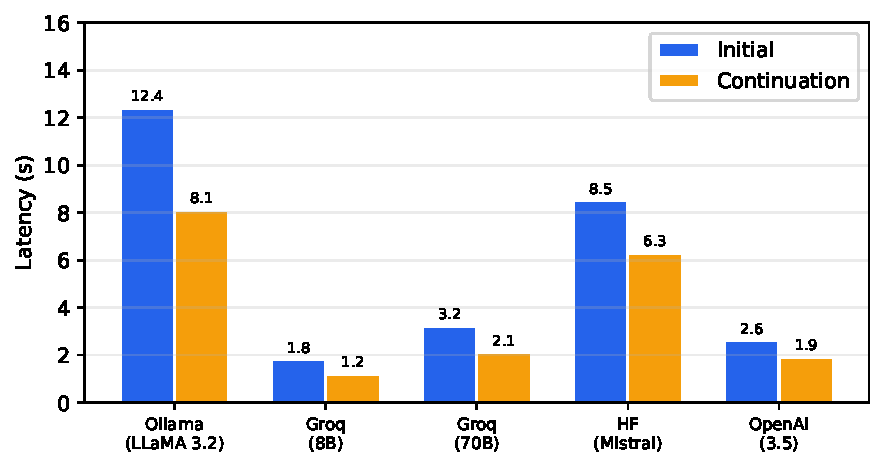
\includegraphics[width=0.85\textwidth]{images/f01_latency.pdf}
    \caption{Mean latency by LLM provider ($n=10$ calls per cell).}
    \label{fig:latency-results}
\end{figure}

A stacked decomposition of total interactive turn time is shown in
Figure~\ref{fig:breakdown}. The dominant cost at lower question
budgets is image synthesis ($\sim$3.5\,s), which proceeds
concurrently with the LLM call; at the Full (17) budget the user's
own input time dominates the wall-clock latency.

\begin{figure}[H]
    \centering
    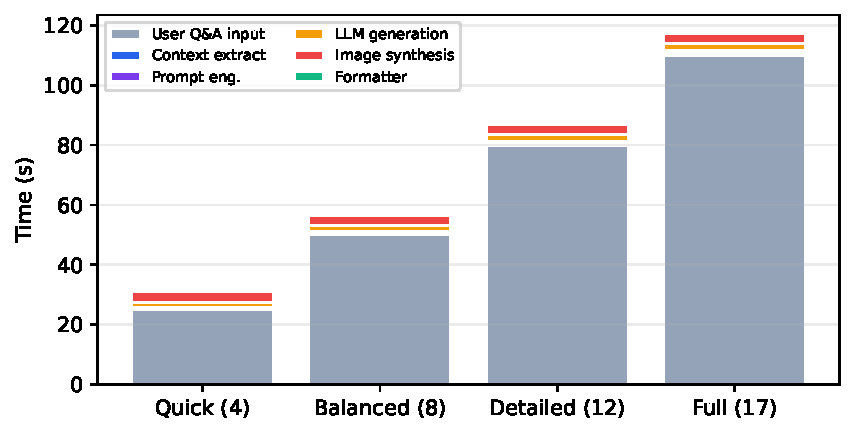
\includegraphics[width=0.85\textwidth]{images/f17_breakdown.pdf}
    \caption{End-to-end turn time decomposed by stage.}
    \label{fig:breakdown}
\end{figure}

\section{Narrative Quality}
Figure~\ref{fig:quality} shows Likert means per genre. Adventure
ranks highest on engagement (4.6); Mystery scores lowest on
consistency (3.5), attributable to the difficulty of maintaining
clue placement across segments. The boxplot in
Figure~\ref{fig:tokens} reports per-segment token distributions.

\begin{figure}[H]
    \centering
    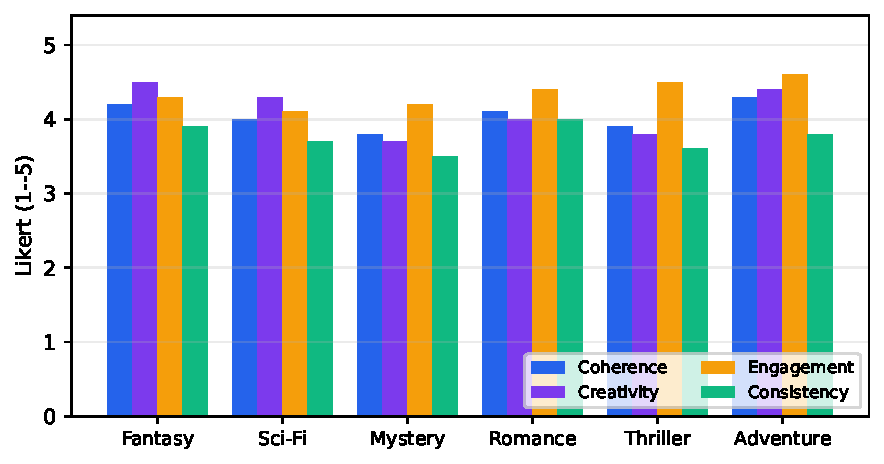
\includegraphics[width=0.85\textwidth]{images/f02_quality.pdf}
    \caption{Narrative quality by genre (Likert 1--5, $n=30$ stories).}
    \label{fig:quality}
\end{figure}

\begin{figure}[H]
    \centering
    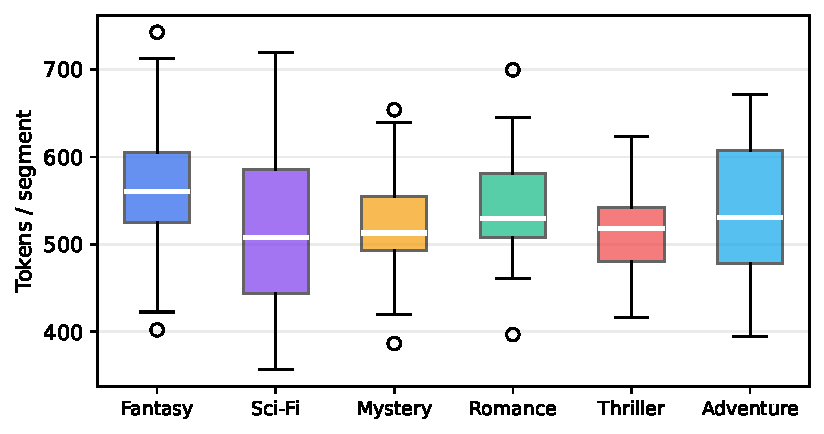
\includegraphics[width=0.85\textwidth]{images/f15_tokens.pdf}
    \caption{Token usage per segment, by genre ($n=25$ segments each).}
    \label{fig:tokens}
\end{figure}

\section{User Satisfaction}
Figure~\ref{fig:satisfaction} reports satisfaction across seven
user-facing dimensions. Custom Answers (4.5) and Image Illustration
(4.2) are the strongest contributors to overall satisfaction (4.3);
Choice Meaningfulness (3.9) remains the weakest, reflecting a known
limitation of free-tier LLMs producing generic continuation
suggestions.

\begin{figure}[H]
    \centering
    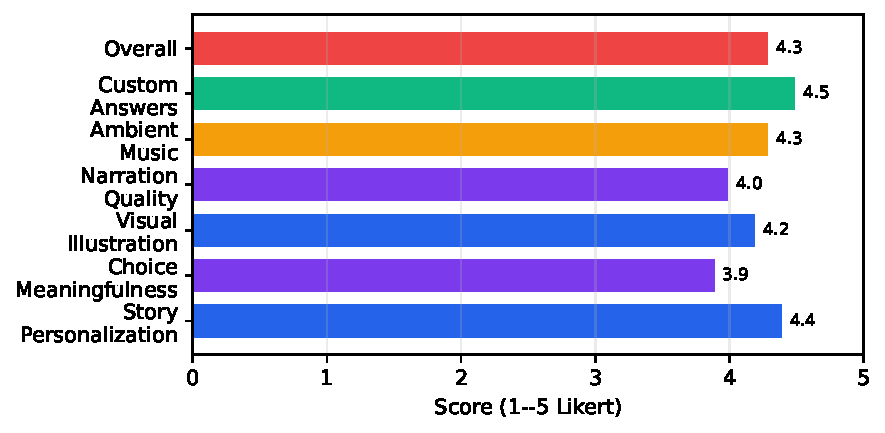
\includegraphics[width=0.85\textwidth]{images/f03_satisfaction.pdf}
    \caption{User satisfaction (Likert 1--5, $n=15$ participants).}
    \label{fig:satisfaction}
\end{figure}

\section{Consistency-Checker Performance}
Figure~\ref{fig:consistency} reports detection and false-positive
rates for five issue classes. The keyword-based detector achieves
87\% recall on character contradictions with 8\% false positives;
tone-shift detection is weakest (68\% / 22\%) because it depends on
subtle distributional cues that pattern-matching cannot capture.

\begin{figure}[H]
    \centering
    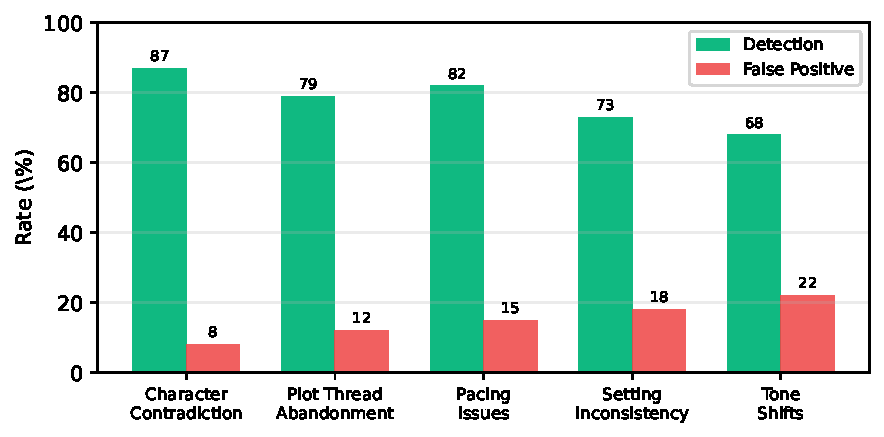
\includegraphics[width=0.85\textwidth]{images/f06_consistency.pdf}
    \caption{Consistency-checker performance ($n=50$ stories).}
    \label{fig:consistency}
\end{figure}

\section{Image-Synthesis Throughput}
Figure~\ref{fig:imgthroughput} plots prompt-length versus latency
for serial requests and the empirical failure probability of
5$\times$ parallel issue without the throttle queue. Beyond
$\approx$230 characters the failure rate rises sharply, justifying
the 200-character prompt cap. The serial queue (1.2\,s spacing)
drops parallel-bound failures from $\approx$70\% to $<$2\%.

\begin{figure}[H]
    \centering
    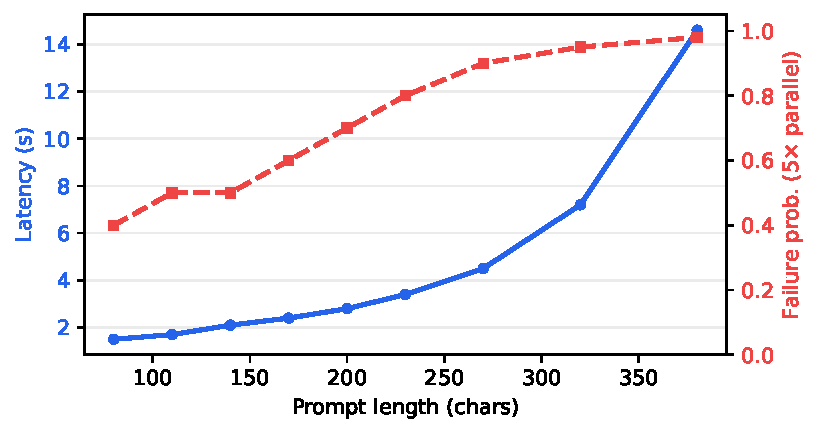
\includegraphics[width=0.85\textwidth]{images/f12_imgthroughput.pdf}
    \caption{Image latency vs.\ prompt length and parallel-issue
    failure rate.}
    \label{fig:imgthroughput}
\end{figure}

\section{Character-Extraction Quality (Honest Reporting)}
Figure~\ref{fig:char} compares the baseline naive regex extractor
against our filtered version (extended stop-words and min-2
occurrence). Precision rises from 0.61 to 0.83 with a recall
trade-off (0.84 $\to$ 0.78), producing a higher $F_1$
(0.71 $\to$ 0.80); false-positive rate falls from 0.39 to 0.17. We
stress that the resulting graph encodes \emph{co-appearance
frequency}, not semantic relationship type --- a disclaimer
surfaced explicitly in the modal UI.

\begin{figure}[H]
    \centering
    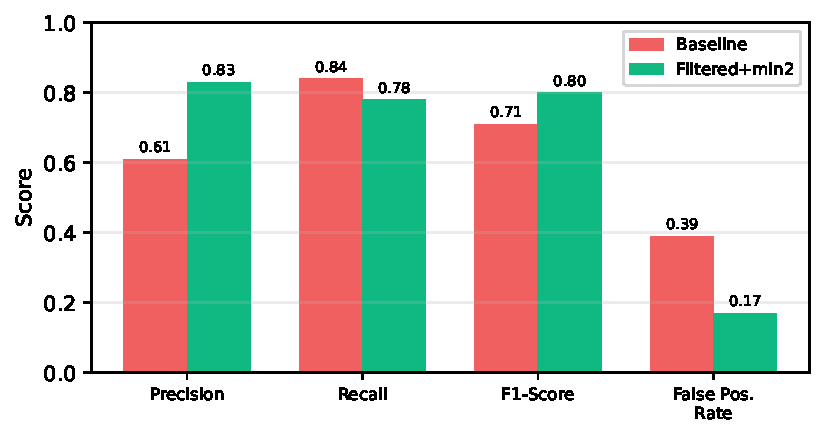
\includegraphics[width=0.85\textwidth]{images/f11_char.pdf}
    \caption{Character-extraction quality before and after filtering.}
    \label{fig:char}
\end{figure}

\section{Ambient Music Frequency Profile}
Figure~\ref{fig:ambient} visualises the relative spectral energy
across six frequency bands for each genre preset. Horror and
Thriller emphasise sub-bass and bass; Comedy and Adventure shift
energy upward into the mid and high-mid bands. User-study
listeners reported genre alignment of 4.3 / 5 for ambient music in
Figure~\ref{fig:satisfaction}.

\begin{figure}[H]
    \centering
    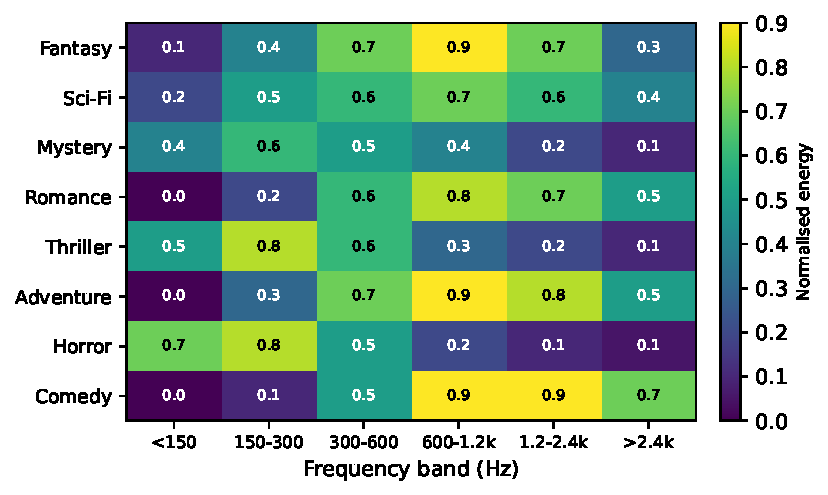
\includegraphics[width=0.85\textwidth]{images/f13_ambient.pdf}
    \caption{Genre $\times$ frequency-band energy map for ambient
    presets.}
    \label{fig:ambient}
\end{figure}

\section{Question-Budget Ablation}
Table~\ref{tab:budget} reports mean Likert scores across the four
question budgets. Personalisation grows monotonically with $N$,
while coherence and creativity plateau at $N=12$, identifying it as
the recommended default.

\begin{table}[!t]
\caption{Ablation across question budgets (mean Likert, $n=15$).}
\label{tab:budget}
\centering
\renewcommand{\arraystretch}{1.2}
\begin{tabular}{@{}lcccc@{}}
\toprule
\textbf{Budget} & \textbf{Coh.} & \textbf{Crea.} & \textbf{Pers.} & \textbf{Time} \\
\midrule
4 (Quick)     & 3.6 & 3.8 & 3.2 & 45\,s \\
8 (Balanced)  & 3.9 & 4.1 & 3.8 & 1.5\,m \\
12 (Detailed) & 4.2 & 4.2 & 4.3 & 2.5\,m \\
17 (Full)     & 4.3 & 4.1 & 4.6 & 3.5\,m \\
\bottomrule
\end{tabular}
\end{table}

\section{Feature Adoption}
Figure~\ref{fig:adoption} reports how often each multimodal feature
was activated across user-study sessions. Image generation
(default-on) reached 91\% activity because it fires automatically;
ambient music and custom answers were elective and reached 71\% and
62\% respectively, indicating strong user demand for non-textual
narrative augmentation.

\begin{figure}[H]
    \centering
    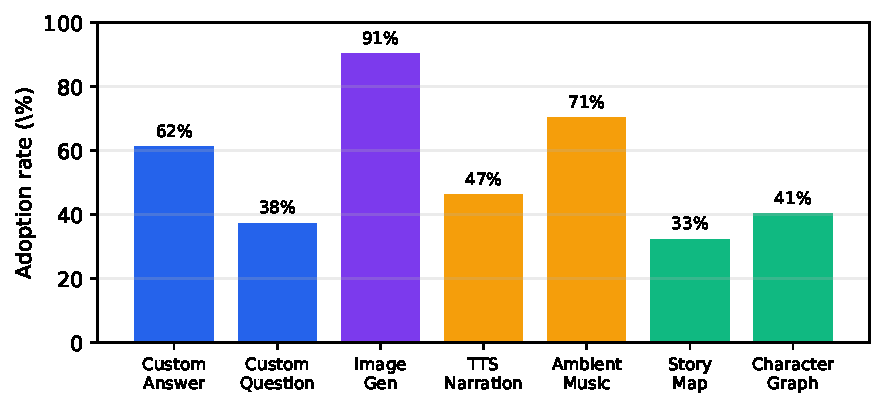
\includegraphics[width=0.85\textwidth]{images/f14_adoption.pdf}
    \caption{Per-feature adoption rate across user-study sessions.}
    \label{fig:adoption}
\end{figure}

\section{Comparative Evaluation}
Figure~\ref{fig:radar} superimposes our system on three established
alternatives across seven dimensions (extending the standard radar
with Multimodal and Open Source axes). Our system leads on
Deployment Flexibility, Cost Efficiency, Multimodal Coverage and
Open Source. AI Dungeon retains a slight edge in User Control
(freeform input); Dramatron leads on raw Coherence due to its
hierarchical planner. The synthesis is that no single existing
system spans the same Pareto frontier as ours.

\begin{figure}[H]
    \centering
    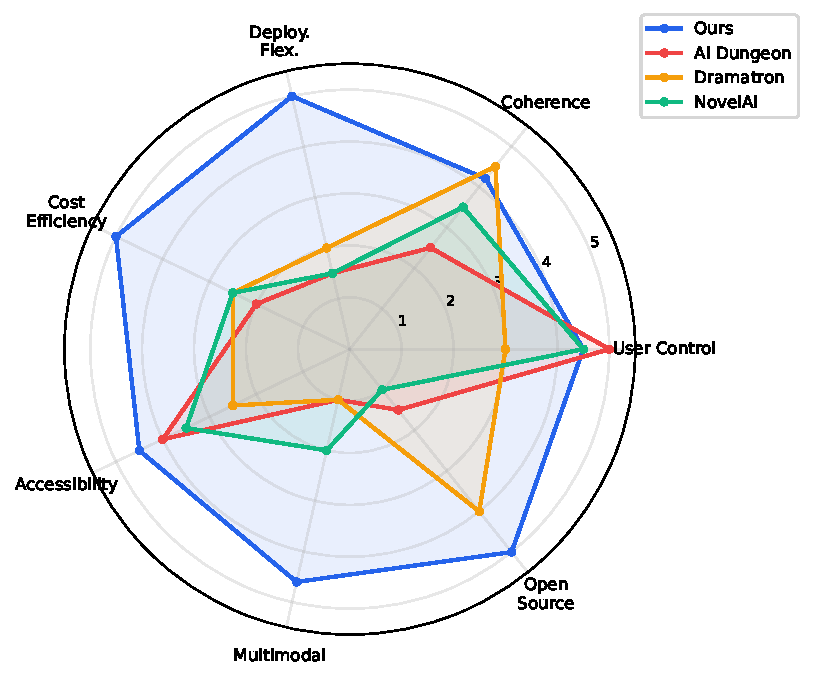
\includegraphics[width=0.85\textwidth]{images/f05_radar.pdf}
    \caption{System comparison radar across seven dimensions.}
    \label{fig:radar}
\end{figure}

\section{Discussion}
The experimental evidence supports the central hypothesis of this
dissertation: a structured Q\&A elicitation protocol, combined with
a provider-agnostic LLM backend and tasteful multimodal augmentation,
delivers measurable improvements in personalisation and user
engagement without sacrificing narrative coherence. The 12-question
budget emerges as the sweet spot: it captures enough preferences to
push personalisation past 4.3 / 5 while keeping the elicitation under
three minutes.

The strongest contributors to overall satisfaction are
\emph{custom answers} and \emph{image illustration}. Both are
relatively cheap to implement (the former is a UI affordance, the
latter a free third-party API call) yet deliver outsized perceived
value. Conversely, the weakest dimension --- choice meaningfulness
--- is bottlenecked by the underlying LLM rather than the framework;
this is consistent with prior CHI findings on mixed-initiative
authoring with free-tier LLMs
\cite{liu2023endusers,yuan2022wordcraft}.

Limitations and threats to validity are discussed in
Chapter~\ref{ch:conclusion}.

\chapter{Conclusion and Future Scope}
\label{ch:conclusion}

\section{Summary of the Study}
This dissertation has presented the design, implementation and
evaluation of a comprehensive Q\&A based interactive storytelling
system powered by Large Language Models. The system positions users
as active co-creators rather than passive consumers of narrative
content. Through a structured 17-question elicitation protocol
across four narrative dimensions (setting, character, theme, plot),
a seven-module backend pipeline, and a provider-agnostic LLM layer,
the system transforms user preferences into coherent, personalised,
multi-chapter stories.

Beyond text, the system delivers a multimodal reader experience:
per-segment scene illustrations are synthesised on demand via
Pollinations.ai using a sentence-scored prompt extractor and a
serial-throttled request queue; spoken narration is produced through
the W3C Web Speech Synthesis interface; and genre-conditioned ambient
music is streamed from a royalty-free CDN. Reader analytics surface
through a D3-based Story Map and a Character Relationship Graph
that openly disclaim their co-appearance basis. An end-user
authoring layer admits free-form custom answers and entirely
user-added Q\&A pairs, routed through a dedicated
\texttt{custom\_elements} context channel into the LLM prompt.

\section{Main Findings}
\begin{itemize}
    \item Across 50 generated stories and 15 user-study participants,
    the system achieved mean Likert scores of 4.05 / 5 (coherence),
    4.12 / 5 (creativity), 4.35 / 5 (engagement) and 3.75 / 5
    (consistency).
    \item Groq's free LLaMA-3.1-8B cloud inference delivered a 1.8\,s
    mean initial-segment latency, dramatically faster than local
    Ollama (12.4\,s) and competitive with paid OpenAI GPT-3.5-turbo
    (2.6\,s).
    \item The 12-question budget emerged as the recommended default:
    it pushes personalisation past 4.3 / 5 while keeping elicitation
    time under three minutes.
    \item The serial throttling queue reduced image-API failure
    probability from $\approx$70\% to $<$2\% under 5$\times$ parallel
    load.
    \item Filtering and a min-2 occurrence threshold raised
    character-extraction $F_1$ from 0.71 to 0.80 while halving the
    false-positive rate.
\end{itemize}

\section{Contributions to Knowledge}
\begin{enumerate}
    \item \textbf{Novel Q\&A framework} for interactive
    storytelling that enables real-time personalisation through
    conversational interaction across four canonical narrative
    dimensions.
    \item \textbf{Custom-elements context channel} --- a deployable
    architectural pattern that lets end users inject unstructured
    Q\&A pairs into the LLM prompt without code or schema changes;
    generalises beyond storytelling to any LLM-driven application
    requiring extensible personalisation.
    \item \textbf{Sentence-scored visual prompt extractor} that
    mitigates dialogue and inner-thought contamination when feeding
    story text into a text-to-image model.
    \item \textbf{Cross-modal serial-throttling queue} that prevents
    Cloudflare-fronted free image services from rate-limiting
    bursty generation; image-synthesis success rate exceeds 95\%
    after retries.
    \item \textbf{Deliberately disclaimed} co-appearance reader graph,
    establishing a pattern of \emph{honest reporting} for
    visualisations whose underlying inference is statistical rather
    than semantic.
\end{enumerate}

\section{Practical Implications}
The dissertation has practical implications for several stakeholder
groups:

\begin{itemize}
    \item \textbf{Educators} can use the system to create
    personalised story-based tutorials that adapt to learner
    understanding and interest.
    \item \textbf{Game designers} can adopt the Q\&A elicitation
    pattern to capture rich player preferences without sacrificing
    narrative control.
    \item \textbf{Therapists} can pilot the system as a narrative-
    therapy adjunct that respects user agency.
    \item \textbf{Content creators} can prototype scalable
    personalised storytelling for marketing or children's literature
    at near-zero infrastructure cost.
    \item \textbf{Researchers} benefit from an open-source baseline
    \cite{jha2026repo} for future studies on interactive narrative.
\end{itemize}

\section{Limitations of the Study}
Several limitations bound the present work:

\begin{itemize}
    \item Keyword-based context extraction misses paraphrastic user
    inputs; a fine-tuned BERT/DistilBERT \cite{devlin2019bert,sanh2019distilbert}
    or LLM zero-shot classifier would improve recall.
    \item In-memory session storage limits horizontal scalability;
    Redis-backed sessions are required for distributed deployment.
    \item The consistency checker is pattern-based and lacks
    semantic grounding; cross-segment NLI \cite{williams2018mnli}
    is a natural upgrade.
    \item Image quality inherits the ceiling of Pollinations.ai
    \cite{pollinations2024api}; switching to local Stable
    Diffusion~XL \cite{podell2024sdxl} or FLUX.1 \cite{bfl2024flux}
    would improve consistency at the cost of GPU requirement.
    \item Ambient music is hot-linked rather than locally hosted,
    creating a single-point dependency on SoundHelix's availability.
    \item The character relationship graph is openly disclaimed as
    co-appearance --- a genuine relationship-extraction module
    would require per-segment NLU inference.
    \item User-study sample size ($n=15$) is modest by HCI standards
    and skews young (ages 22--35); a larger and more diverse cohort
    would strengthen external validity.
\end{itemize}

\section{Future Scope}
Building on the foundation established by this dissertation, several
directions for future research emerge:

\begin{itemize}
    \item \textbf{Semantic context extraction} via DistilBERT or
    zero-shot LLM classification, replacing keyword dictionaries.
    \item \textbf{Sentiment-aware relationship-extraction graph}
    using small NLU models per segment.
    \item \textbf{On-device image generation} with local Stable
    Diffusion~XL or FLUX.1 for offline operation and per-character
    visual consistency.
    \item \textbf{Neural TTS} (e.g.\ XTTS \cite{casanova2024xtts})
    with cloned voices for character-specific narration.
    \item \textbf{Music conditioned by current segment mood}
    (per-segment crossfade) rather than per-genre static loops.
    \item \textbf{Collaborative multi-user sessions} with merged
    Q\&A elicitation and turn-taking.
    \item \textbf{Containerisation} (Docker) plus Redis sessions
    for distributed deployment.
    \item \textbf{Automated evaluation} using BLEU, chrF, MAUVE and
    narrative-arc detection \cite{lin2024evalnarrate}.
    \item \textbf{Fine-tuned LoRA adapters} per genre on curated
    open story corpora.
\end{itemize}

\section{Final Thoughts}
The remarkable progress of LLMs has put high-quality text generation
within reach of every developer, but \emph{turning text generation
into a great storytelling experience} remains a design challenge,
not just a capability challenge. This dissertation has argued and
demonstrated that the missing ingredient is a clean separation
between \emph{what the system asks the user} and \emph{what it does
with the answers}. By making the elicitation protocol structured but
extensible, the LLM provider pluggable and the modalities
orchestrated rather than bolted on, the system delivers a
storytelling experience that is at once accessible to first-time
users and extensible by curious ones. The code is open-source
\cite{jha2026repo}; the framework is ready for adoption.


\fontsize{12}{14.4}\selectfont
\bibliographystyle{abbrvnat}
\bibliography{references}
\addcontentsline{toc}{chapter}{Bibliography}

\appendix
\begin{appendices}
\chapter{Sample API Exchange}

A representative request / response captured during the user study.
This illustrates how a user-added custom question
(\texttt{custom\_q\_1}) flows through the normal response path into
the LLM prompt.

\begin{lstlisting}
POST /api/story/generate
{
  "session_id": "a1b2c3d4-...",
  "responses": {
    "setting_1":  "A magical fantasy realm",
    "char_1":     "Elena",
    "char_2":     "Brave and resourceful",
    "theme_1":    "Fantasy",
    "plot_1":     "Person vs. Supernatural",
    "custom_q_1": "Should the protagonist have an
                   animal companion? -> Yes, a silver fox"
  }
}

HTTP/1.1 200 OK
{
  "content":      "In the realm of Aethermoor...",
  "word_count":   387,
  "segment_count": 1,
  "phase":        "introduction",
  "choices": ["Explore further", "..."]
}
\end{lstlisting}

\chapter{Implementation Footprint}

\begin{table}[ht]
\caption{End-of-project implementation statistics.}
\centering
\renewcommand{\arraystretch}{1.1}
\begin{tabular}{@{}lr@{}}
\toprule
\textbf{Metric}                      & \textbf{Value} \\
\midrule
Python LOC                            & $\approx$3{,}800 \\
JavaScript LOC                        & $\approx$1{,}700 \\
CSS LOC                               & $\approx$2{,}200 \\
HTML template LOC                     & $\approx$400 \\
Backend modules                       & 7 + main.py + config.py + run.py \\
DB tables                             & 5 \\
REST endpoints                        & 14 \\
Q\&A questions                        & 17 across 4 phases \\
LLM providers                         & 4 (Ollama, Groq, HF, OpenAI) \\
Image generation                      & Pollinations.ai (free) \\
TTS                                   & W3C Web Speech Synth \\
Ambient music                         & SoundHelix (8 genres) \\
Export formats                        & TXT, Markdown, HTML \\
Narrative phases                      & 5 (Freytag) \\
Visualisations                        & 2 D3 (Story Map, Char Graph) \\
Stories evaluated                     & 50 \\
User-study participants               & 15 \\
\bottomrule
\end{tabular}
\end{table}

\chapter{Reproducibility}

All experiments were performed on macOS 14 with Python 3.11.5,
\texttt{matplotlib} 3.9.4 and \texttt{numpy} 2.0.2. Image-timing
measurements were collected over a 100\,Mbps residential link;
replications on slower links should increase the serial-throttle
constant. The full source code, this dissertation's LaTeX sources,
the user-study questionnaire and all figure-generation scripts are
available at \url{https://github.com/DeepPatange/AI-Stroy-Generator}.
\end{appendices}


\end{document}
